%%%%%%%%%%%%%%%%%%%%%%%%%%%%%%%%%%%%%%%%%%%%%%%%%%%%%%%%%%%%%%%%%%%
%                                                                 %
%  GEANT manual in LaTeX form                                     %
%                                                                 %
%  Version 1.00                                                   %
%                                                                 %
%  Last Mod. 8 June 1993  17:20  MG                               %
%                                                                 %
%%%%%%%%%%%%%%%%%%%%%%%%%%%%%%%%%%%%%%%%%%%%%%%%%%%%%%%%%%%%%%%%%%%
\documentstyle[11pt,fleqn,epsfig,crngeant,bibunits,fontcmds,multicol]{cernman}
\newcommand{\Title}{GEANT User's Guide}%           Title for document
\psfigdriver{DVIPS}
\makeindex
\romanfont{times}
\PScommands% Initialize PS boxes
\newmathalphabet*{\mathtt}{cmtt}{m}{n}
\newmathalphabet*{\mathbf}{cmr}{b}{n}
\begin{document}
%  ==================== Front material ============================
%%%%%%%%%%%%%%%%%%%%%%%%%%%%%%%%%%%%%%%%%%%%%%%%%%%%%%%%%%%%%%%%%%%
%                                                                 %
%   GEANT -- Short write ups -- LaTeX Source                      %
%                                                                 %
%   Front Material: Title page,                                   %
%                   Copyright Notice                              %
%                   Preliminary Remarks                           %
%                   Table of Contents                             %
%   EPS file      : cern15.eps, cnastit.eps                       %
%                                                                 %
%   Editor: Michel Goossens / CN-AS                               %
%   Last Mod.: 11 June 1993 10:30 mg                              %
%                                                                 %
%%%%%%%%%%%%%%%%%%%%%%%%%%%%%%%%%%%%%%%%%%%%%%%%%%%%%%%%%%%%%%%%%%%
 
%%%%%%%%%%%%%%%%%%%%%%%%%%%%%%%%%%%%%%%%%%%%%%%%%%%%%%%%%%%%%%%%%%%%
%    Tile page                                                     %
%%%%%%%%%%%%%%%%%%%%%%%%%%%%%%%%%%%%%%%%%%%%%%%%%%%%%%%%%%%%%%%%%%%%
\latex{\def\Ptitle#1{\special{ps: /Printstring (#1) def}
                       \epsfbox{eps/cnastit.eps}}}
 
\begin{titlepage}
%begin{latexonly}
\vspace*{-23mm}%

\includegraphics[height=30mm]{cern.eps}
\hfill
\raise8mm\hbox{\Large\bf CERN Program Library Long Writeup W5013}
\hfill\mbox{}
\begin{center}
\mbox{}\\[6mm]
\mbox{\Ptitle{GEANT}}\\[3cm]
{\Huge Detector Description and}\\[2cm]
{\Huge Simulation Tool}\\[4cm]
{\Large Application Software Group}\\[6mm]
{\Large Computing and Networks Division}\\[2cm]
\end{center}
\vfill
\begin{center}\Large CERN Geneva, Switzerland\end{center}
%end{latexonly}
\begin{htmlonly}
\begin{center}
\Large CERN Program Library Long Writeup W5013\\[1cm]
\Huge GEANT\\[2cm]
\Large Detector Description and Simulation Tool\\[1cm]
\large IT/ASD Group\\
\large CERN, Geneva, Switzerland
\end{center}
\end{htmlonly}
\end{titlepage}

%%%%%%%%%%%%%%%%%%%%%%%%%%%%%%%%%%%%%%%%%%%%%%%%%%%%%%%%%%%%%%%%%%%%
%    Copyright  page                                               %
%%%%%%%%%%%%%%%%%%%%%%%%%%%%%%%%%%%%%%%%%%%%%%%%%%%%%%%%%%%%%%%%%%%%

\thispagestyle{empty}
\framebox[\textwidth][t]{\hfill\begin{minipage}{0.96\textwidth}%
\vspace*{3mm}
\begin{center}Copyright Notice\end{center}
\parskip\baselineskip

\textbf{GEANT -- Detector Description and Simulation Tool}
 
\copyright{} Copyright CERN, Geneva 1993
 
Copyright and any other appropriate legal protection of these
computer programs and associated documentation reserved in all
countries of the world.
 
These programs or documentation may not be reproduced by any
method without prior written consent of the Director-General
of CERN or his delegate.
 
Permission for the usage of any programs described herein is
granted apriori to those scientific institutes associated with
the CERN experimental program or with whom CERN has concluded
a scientific collaboration agreement.
 
CERN welcomes comments concerning the Geant code
but undertakes no obligation for the maintenance of the programs,
nor responsibility for their correctness, and accepts no liability
whatsoever resulting from the use of its programs.
 
Requests for information should be addressed to:
\vspace*{-.5\baselineskip}
\begin{center}\ttfamily
\begin{tabular}{l}
CERN Program Library Office              \\
CERN-IT Division                         \\
CH-1211 Geneva 23                        \\
Switzerland                              \\
Tel.      +41 22 767 4951                \\
Fax.      +41 22 767 7155                \\
Email:    cernlib@cern.ch                \\
WWW:      http://wwwinfo.cern.ch/asd/index.html
\end{tabular}
\end{center}
\vspace*{2mm}
\end{minipage}\hfill}%end of minipage in framebox
\vspace{6mm}
 
{\bf Trademark notice: All trademarks appearing in this guide are acknowledged as such.}
\vfill

\begin{tabular}{l@{\quad}l@{\quad}>{\small\ttfamily}l}
\emph{Contact Persons}:       & IT/ASD/SImulation section & (giani\atsign cern.ch)\\[1mm]
\emph{Documentation Consultant}: & Michel Goossens /IT    & (goossens\atsign cern.ch)\\[1cm]
\textem{Edition -- March 1994}
\end{tabular}
\newpage
 

%  ==================== Body of text ==============================
\pagenumbering{arabic}
\setcounter{page}{1}
 
%%%%%%   Catalog of Program packages and entries%%%%
 
\def\Rtnr{Catalog}%Dummy routine name to appear at bottom of page
%%%%%%%%%%%%%%%%%%%%%%%%%%%%%%%%%%%%%%%%%%%%%%%%%%%%%%%%%%%%%%%%%%%
%                                                                 %
%  GEANT manual in LaTeX form   	                          %
%                                                                 %
%  Michel Goossens (for translation into LaTeX)                   %
%  Version 2.00                                                   %
%  Last Mod.  2 Jun 1998  17:10   MG                              %
%                                                                 %
%%%%%%%%%%%%%%%%%%%%%%%%%%%%%%%%%%%%%%%%%%%%%%%%%%%%%%%%%%%%%%%%%%%
%%% Generated from headings
\chapter{Catalog of Geant sections}
\begin{DLtt}{12345678}
\item[AAAA001] Foreword
\item[AAAA002] Introduction to the manual
\item[BASE001] Introduction to GEANT
\item[BASE010] Simplified Program Flow Chart
\item[BASE020] The data structures and their relationship
\item[BASE040] Summary of Data Records
\item[BASE090] The reference systems and physical units
\item[BASE100] Examples of GEANT application
\item[BASE110] The system initialisation routines
\item[BASE200] Steering routines for event processing
\item[BASE280] Storing and retrieving JRUNG and JHEAD information
\item[BASE299] The banks JRUNG and JHEAD
\item[BASE300] Example of user termination routine
\item[BASE400] Debugging facilities
\item[BASE410] Utility Routines
\item[BASE420] The random number generator
\item[CONS001] Introduction to the section CONS
\item[CONS100] Material definition
\item[CONS101] Retrieve material cross-sections and stopping power
\item[CONS110] Mixtures and Compounds
\item[CONS199] The Material data structure JMATE
\item[CONS200] Tracking medium parameters
\item[CONS210] Special Tracking Parameters
\item[CONS300] Particle definition
\item[CONS310] Branching Ratios and Particle Decay Modes
\item[DRAW001] Introduction to the Drawing package
\item[DRAW010] The Ray-tracing package
\item[DRAW110] Drawing a Volume -- Case 1
\item[DRAW115] Drawing a Volume Projection view -- Case 2
\item[DRAW120] Draw a volume cut view
\item[DRAW130] Draw Particle Trajectories
\item[DRAW140] Drawing Track Hits in Sensitive Detectors
\item[DRAW210] Drawing the geometrical tree
\item[DRAW220] Drawing volume specifications
\item[DRAW300] Handling View banks
\item[DRAW399] The data structure JDRAW
\item[DRAW400] Utility routines of the drawing package
\item[GEOM001] The geometry package
\item[GEOM010] Tracking inside volumes and optimisation
\item[GEOM020] ``MANY'' Volumes and boolean operations on volumes
\item[GEOM050] The GEANT shapes
\item[GEOM100] Creation of a volume
\item[GEOM110] Positioning a volume inside its mother
\item[GEOM120] Positioning a volume inside its mother with parameters
\item[GEOM130] Division of a volume into a given number of cells
\item[GEOM140] Division of a Volume into cells of a given size
\item[GEOM150] Division of a volume - general case
\item[GEOM199] The volume data structure -- JVOLUM
\item[GEOM200] Rotation matrices
\item[GEOM299] The rotation matrix data structure JROTM
\item[GEOM300] Finding in which volume a point is
\item[GEOM310] Finding distance to next boundary
\item[GEOM320] Reference system transformations
\item[GEOM400] Pseudo-division of a volume
\item[GEOM410] Ordering the contents of a volume
\item[GEOM500] Volume attributes
\item[GEOM600] User initialisation of the common block /GCVOLU/
\item[GEOM700] Medium search statistics
\item[GEOM900] End of geometry definition
\item[GEOM910] The CADINT Interface
\item[HITS001] The detector response package
\item[HITS100] Sensitive DETector definition
\item[HITS105] Detector aliases
\item[HITS110] DETector hit parameters
\item[HITS120] DETector Digitisation parameters
\item[HITS130] User detector parameters
\item[HITS199] The SET data structure JSET
\item[HITS200] Routines to store and retrieve HITS
\item[HITS299] The JHITS data structure
\item[HITS300] Routines to store and retrieve DIGItisations
\item[HITS399] The JDIGI data structure
\item[HITS400] Intersection of a track with a cylinder or a plane
\item[HITS500] Digitisation for drift- or MWP- Chambers
\item[HITS510] Digitisation for drift chambers
\item[IOPA001] The I/O routines
\item[IOPA200] ZEBRA sequential files handling
\item[IOPA300] Data structure I/O with sequential files
\item[IOPA400] ZEBRA direct access files handling
\item[IOPA500] Data structure I/O with direct access files
\item[KINE001] Section KINE
\item[KINE100] Storing and retrieving vertex and track parameters
\item[KINE199] The data structures JVERTX and JKINE
\item[KINE200] Interface to the Lund Monte Carlo
\item[KINE210] $\tau ^{\pm }$ generation and decay
\item[PHYS001] Introduction to the section PHYS
\item[PHYS010] Compute the occurrence of a process
\item[PHYS100] Steering routine for physics initialisation
\item[PHYS210] Total cross-section for e+e- pair production by photons
\item[PHYS211] Simulation of e-e+ pair production by photons
\item[PHYS220] Total cross-section for Compton scattering
\item[PHYS221] Simulation of Compton scattering
\item[PHYS230] Total cross-section for photoelectric effect
\item[PHYS231] Simulation of photoelectric Effect
\item[PHYS240] Photon-induced fission on heavy materials
\item[PHYS250] Total cross-section for Rayleigh scattering
\item[PHYS251] Simulation of Rayleigh scattering
\item[PHYS260] \v{C}erenkov photons
\item[PHYS320] Gaussian multiple scattering
\item[PHYS325] Moli\`ere scattering
\item[PHYS328] Plural scattering
\item[PHYS330] Ionisation processes induced by e+/e-
\item[PHYS331] Simulation of the delta-ray production
\item[PHYS332] Simulation of energy loss straggling
\item[PHYS333] Information about energy loss fluctuations
\item[PHYS334] Models for energy loss fluctuations in thin layers
\item[PHYS337] Birks' saturation law
\item[PHYS340] Total cross-section and energy loss for bremsstrahlung by e-e+
\item[PHYS341] Simulation of discrete bremsstrahlung by electrons
\item[PHYS350] Total cross-section for e+e- annihilation
\item[PHYS351] Simulation of e+e- annihilation
\item[PHYS360] Synchrotron radiation
\item[PHYS400] Simulation of particle decays in flight
\item[PHYS410] Rotations and Lorentz transformation
\item[PHYS430] Ionisation processes for muons and protons
\item[PHYS431] Ionisation processes for heavy ions
\item[PHYS440] Total cross-section and energy loss for bremsstrahlung by Muons
\item[PHYS441] Simulation of discrete bremsstrahlung by muons
\item[PHYS450] Total cross-section and energy loss for e-e+ pair production by muons
\item[PHYS451] Simulation of e+e- pair production by muons
\item[PHYS460] Muon-nucleus interactions
\item[PHYS510] The GEANT/GHEISHA Interface
\item[PHYS520] The GEANT/FLUKA Interface
\item[PHYS530] The GEANT/MICAP interface
\item[TRAK001] The tracking package
\item[TRAK110] Steering routine to track one event
\item[TRAK120] Steering routine to track one particle
\item[TRAK130] Tracking one particle through a volume
\item[TRAK200] The tracking routines block diagrams
\item[TRAK300] Storing secondary tracks in the stack
\item[TRAK310] Altering the order of tracking secondary particles
\item[TRAK399] The temporary stack data structure JSTAK
\item[TRAK400] Handling of track space points
\item[TRAK499] The space point data structure JXYZ
\item[TRAK500] Tracking routines in magnetic field
\item[XINT001] The interactive version of GEANT
\item[XINT002] Introduction to the Interactive version of GEANT
\item[XINT010] Screen views of GEANT++
\item[ZZZZ010] List of COMMON Blocks
\item[ZZZZ999] Index of Documented GEANT routines
\end{DLtt}

 
\let\LARGE\large
\let\Large\large
\let\DL\DLtt 

% Here come the different files to be included
 
%%     BASE part     %%

\begin{bibunit}[unsrt]
\renewcommand{\bibname}{BASE Bibliography}
\cleardoublepage
%%%%%%%%%%%%%%%%%%%%%%%%%%%%%%%%%%%%%%%%%%%%%%%%%%%%%%%%%%%%%%%%%%%
%                                                                 %
%  GEANT manual in LaTeX form                                     %
%                                                                 %
%  Michel Goossens (for translation into LaTeX)                   %
%  Version 1.00                                                   %
%  Last Mod. Jan 24 1991  1300   MG + IB                          %
%                                                                 %
%%%%%%%%%%%%%%%%%%%%%%%%%%%%%%%%%%%%%%%%%%%%%%%%%%%%%%%%%%%%%%%%%%%
\Documentation {F.Bruyant}       \Origin{GEANT}
\Submitted{01.10.84}       \Revised{08.11.93}
\Version{Geant 3.16}\Routid{BASE001}
\Makehead{Introduction to GEANT}
\section{{\tt GEANT} applications}
 
The {\tt GEANT} program simulates the passage of elementary particles through
the matter. Originally designed for the High Energy Physics experiments,
it has today found applications also outside this domain in areas such as
medical and biological sciences, radio-protection and astronautics.

The principal applications of {\tt GEANT} in High Energy Physics are:
\begin{itemize}
\item the {\it transport} 
of particles ({\it tracking} in this manual)
through an experimental setup for the simulation
of detector response;
\item
the graphical representation of the setup and of the particle trajectories.
\end{itemize}

The two functions are combined in the interactive version of {\tt GEANT}.
This is very useful,
since the direct
observation of what happens to a particle inside the detector
makes the debugging easier and may reveal possible weakness of the
setup (also sometimes of the program!).

In view of these applications, the {\tt GEANT} system allows you to:
\begin{itemize}
\item
describe an experimental setup
by a structure of geometrical volumes.
A {\tt MEDIUM} number 
is assigned to each volume
by the user ({\tt [GEOM]}). Different volumes may have
the same medium number. A medium is defined by
the so-called {\tt TRACKING MEDIUM} parameters, which
include reference to the {\tt MATERIAL}
filling the volume {\tt [CONS]};
\item
accept events simulated by Monte Carlo generators {\tt [KINE]};
\item transport particles through the various
regions of the setup, taking
into account geometrical volume boundaries and
physical effects according to the nature of the
particles themselves, their interactions
with matter and the magnetic field {\tt [TRAK], [PHYS]};
\item
record particle trajectories and the response of
the sensitive detectors {\tt [TRAK], [HITS]};
\item visualise the
detectors and the particle trajectories {\tt [DRAW], [XINT]}.
\end{itemize}

The program contains {\it dummy} and {\it default}
user subroutines called whenever application-dependent
actions are expected.

It is the responsibility of the user to:
\begin{itemize}
\item code the relevant user subroutines providing the data describing the
experimental environment;
\item assemble the appropriate program segments and utilities into an 
executable program;
\item compose the appropriate data records
which control the execution of the program. 
\end{itemize}
The
section {\tt [BASE]} of this manual gives more information on the above.

{\bf Note:}
the names of the dummy or default user subroutines have {\tt GU} or {\tt UG} 
as their first two letters.
 
\section{Event simulation framework}

The framework offered by {\tt GEANT} for event simulation is described in
the following paragraphs, in order
to familiarise the reader with the areas where user
interventions are expected.
For each item we will indicate in brackets the relevant section where more
information can be found.

At the same time, the {\tt GEANT} data structures are introduced. 
This is
important as the coding to be provided by the user
most often consists of storing and retrieving information from
data structures, or reading or writing data structures.
For simple applications
user routines are provided as an interface to the data structures
partially hiding them from the users. For advanced users of 
{\tt GEANT}, some idea of the layout of the data in memory is helpful.
{\tt GEANT} data structures are logically related set of data which are
physically stored in the \FCind{/GCBANK/} common block. The position
of each structure is contained in an {\tt INTEGER} variable which
is constantly kept up-to-date by {\tt ZEBRA}. By convention the names
of these variable, called {\it pointers} begin with {\tt J}, and they
are used in this manual to designate the structure they point to.

A main program has to be provided by the user ({\tt [BASE100]}) for
{\it batch} type operation. For interactive operation a main program is
provided, both binary and source, in the library directory
both at CERN and in the standard distribution tape of the CERN Program
Library. The file is called {\tt gxint<ver>.<ext>}, where {\tt <ver>}
is the version of {\tt GEANT} to which this file belongs and {\tt <ext>}
is the system-dependent file-name extension to denote a FORTRAN source
or an object file. This file should be loaded in front of all other
files when assembling a {\tt GEANT} application. The source is provided
in case the user wants to modify it, in particular changing the size
of the commons \FCind{/GCBANK/} or \FCind{/PAWC/}.

The main program allocates the dynamic memory for {\tt ZEBRA} and 
{\tt HBOOK} and passes control to the three phases of the run:
 
\begin{enumerate}
\item initialisation
\item event processing
\item termination
\end{enumerate}

where in each of the three phases the user can implement his own code
in the appropriate routines.
 
\section{Initialisation}

The initialisation is controlled by the user in the subroutine {\tt UGINIT}  
who has the responsibility to call the appropriate routines
({\tt [BASE100]}).
It consists of the following steps, most of them
performed through calls to {\tt GEANT} subroutines:
 
\begin{DLtt}{MMMMMMMMMM}
\item[\Rind{GINIT}]
initialise the {\tt GEANT} common blocks
with default values ({\tt [BASE030], [BASE110]});
\item[\Rind{GFFGO}]
read {\it free format} data records either to
modify the default options ({\tt [BASE040],
[BASE110]}) or to provide information on the current run;
\item[\Rind{GZINIT}]
initialise the memory manager, the link areas
and the run header bank {\tt JRUNG} ({\tt [BASE110]});
\item[\Rind{GDINIT}]
initialise the drawing package ({\tt [DRAW]}), calling this routine
without having initialised the graphics package via a call to \Rind{IGINIT}
or \Rind{HPLINT} will cause {\tt GEANT} to abort;
\item[\Rind{GPART}]
(or \Rind{GSPART}) fill the data structure {\tt JPART}
with the particle properties ({\tt [CONS]});
\item[\Rind{GMATE}] (or \Rind{GSMATE})
fill the data structure {\tt JMATE}
with the characteristics of the materials used
({\tt [CONS]});
\item[User code] it is the responsibility of the user to:
\begin{itemize}
\item define the geometry of the different components of
the setup ({\tt [GEOM]}), stored in the {\tt JROTM} and {\tt JVOLUM} data
structures; 
\item define tracking medium parameters ({\tt [CONS],[TRAK]}), stored
in the {\tt JTMED} data structure;
\item specify which elements of the geometrical
setup should be considered as {\it sensitive detectors}, giving
a {\it response} when hit by a particle ({\tt [HITS]});
\item usually all done in a user routine called \Rind{UGEOM};
\end{itemize}
\item[\Rind{GGCLOS}]
process all the geometrical information
provided by the user and prepare for particle transport;
\item[\Rind{GBHSTA}]
book standard {\tt GEANT} histograms if required by
the user with the data record {\tt HSTA} ({\tt [BASE040], [BASE110]});
\item[\Rind{GPHYSI}]
compute energy loss and cross-section tables
and store them in the data structure {\tt JMATE} ({\tt [CONS], [PHYS]}).
\end{DLtt}
 
\section{Event processing}
 
The processing phase is triggered by a call to the subroutine \Rind{GRUN} which,
for each event to be processed, gives control to the subroutines:
 
\begin{DLtt}{MMMMMMMM}
\item[\Rind{GTRIGI}] initialise event processing and create the
event header bank {\tt JHEAD};
\item[\Rind{GTRIG}] process one event;
\item[\Rind{GTRIGC}] clean up the portion of memory used by the event
and check that enough time is left for the next event ({\tt [BASE200]}).
\end{DLtt}
\Rind{GTRIG} calls the following user routines:
\begin{DLtt}{MMMMMMMM}
\item[\Rind{GUKINE}]
generates or reads ({\tt [IOPA]})
the kinematics of the event and stores it
in the data structures {\tt JVERTX} and {\tt JKINE} ({\tt [KINE]});

\item[\Rind{GUTREV}]
calling \Rind{GTREVE} which performs the following operations for each
vertex in turn:
\begin{enumerate}
\item moves all the particles attached to the vertex from the permanent 
stack {\tt JKINE} to the temporary stack {\tt JSTAK};
\item controls the propagation of each particle though the setup by 
calling \Rind{GUTRAK}/\Rind{GTRACK} ({\tt [TRAK]}); 
each particle is tracked in turn and when a sensitive detector
is traversed, the user may store
any useful information in the data structure {\tt JHITS} 
via the routines described in the section {\tt [HITS]};
\end{enumerate}
 
The {\tt JSTAK} data structure is a LIFO (Last In -- First Out) stack.
Secondary products generated by the current particle transported
are processed before proceeding to the next particle. 
It is very important to understand that by default {\tt GEANT} does not
follow the secondary particles generated. It is the responsibility of the
user to indicate which particles should be followed via the
routines \Rind{GSKING}/\Rind{GSKPHO}.

The data structure {\tt JXYZ}, containing the
coordinates of space points along the tracks,
can be filled by the user during tracking ({\tt [TRAK]}).

\item[\Rind{GUDIGI}]
simulate the detector responses for the event, using 
the information recorded in the data
structure {\tt JHITS} during particle transport, and store
the results in the data structure {\tt JDIGI} ({\tt [HITS]});

\item[\Rind{GUOUT}]
perform all the processing at the end of the event and 
output the relevant data structures ({\tt [IOPA]}).
\end{DLtt}
 
Other routines called during the tracking phase triggered
by {\tt GTREVE} should be mentioned for completeness:
\begin{itemize}
\item
hadronic interactions can be simulated via either the 
{\tt GHEISHA}~\cite{bib-GHEI} or 
{\tt FLUKA}~\cite{bib-FLUK,bib-FLU1,bib-FLU2,bib-FLU3,bib-FLU4}
hadronic shower generator.
In the
subroutines \Rind{GUPHAD} and \Rind{GUHADR} ({\tt [TRAK]}) the user
may select the hadronic shower generation program to be used.
The default for {\tt GEANT} is {\tt GHEISHA};
\item after each tracking step along the
track, control is
given to the subroutine \Rind{GUSTEP}. From the information
available in labelled common blocks the user
is able to take the appropriate action, such as
storing a hit or transferring a secondary product either in the
stack {\tt JSTAK} or in the event structure {\tt JVERTX/JKINE} via
the subroutine 
\Rind{GSKING}. In the subroutine \Rind{GSSTAK},
called by \Rind{GSKING}, a user routine \Rind{GUSKIP} is called which permits
skipping any unwanted track before entering it in the stack for subsequent
transport;
\item the subroutine
\Rind{GUSWIM} is called by the the routines which transport charged particles
when in a magnetic field; it selects and calls the appropriate routine to
transport the particle. Although formally a user routine, the default version
provided by {\tt GEANT} is usually appropriate for most situations.
The magnetic field, unless it is constant along the {\tt Z} axis,
has to be described via the subroutine \Rind{GUFLD}.
\end{itemize}
 
\section{Termination}
 
The termination phase is under the control of the user ({\tt [BASE300]})
via the routine \Rind{GULAST}. In 
simple cases it may consist of a call to the subroutine \Rind{GLAST} 
which computes and prints some statistical information (time per
event, use of dynamic memory, etc.).

%%%%%%%%%%%%%%%%%%%%%%%%%%%%%%%%%%%%%%%%%%%%%%%%%%%%%%%%%%%%%%%%%%%
%                                                                 %
%  GEANT manual in LaTeX form                                     %
%                                                                 %
%  Version 1.00                                                   %
%                                                                 %
%  Last Mod. 19 Oct  1994 18:40 MG                                %
%                                                                 %
%%%%%%%%%%%%%%%%%%%%%%%%%%%%%%%%%%%%%%%%%%%%%%%%%%%%%%%%%%%%%%%%%%%
\Documentation {F.Bruyant, S.Ravndal}       
\Submitted{01.10.84}          \Revised{19.10.94}
\Version{Geant 3.16}\Routid{BASE010}
\Makehead{Simplified Program Flow Chart}


\begin{tabbing}

123\= 123\= 123\= 123\= 123\= 123\= 123\= 123\= 123123123123123123123123\= \kill

MAIN \> \> \> \> \> \> \> \> \> \parbox[t]{7.5cm}{user routine
\vspace{.20cm}} \\
   \> GZEBRA \> \> \> \> \> \> \> \> \parbox[t]{7.5cm}{initialisation of
ZEBRA system, dynamic core allocation \vspace{.20cm}} \\
  \> UGINIT \> \> \> \> \> \> \> \> \parbox[t]{7.5cm}{user routine
\vspace{.20cm}} \\
  \> \> GINIT \> \> \> \> \> \> \> \parbox[t]{7.5cm}{initialisation of
{\tt GEANT} variables \vspace{.20cm}} \\
  \> \> GFFGO \> \> \> \> \> \> \> \parbox[t]{7.5cm}{interpretation of
data records \vspace{.20cm}} \\
  \> \> GZINIT \> \> \> \> \> \> \> \parbox[t]{7.5cm}{initialisation of
ZEBRA core divisions and link areas \vspace{.20cm}} \\
  \> \> GPART/GSPART \> \> \> \> \> \> \> \parbox[t]{7.5cm}{creation of the
{\em particle} data structure {\tt JPART} \vspace{.20cm}} \\
  \> \> GMATE/GSMATE \> \> \> \> \> \> \> \parbox[t]{7.5cm}{creation of the {\em
material} \vspace{.20cm} data structure {\tt JMATE} } \\
  \> \> {\em user code} \> \> \> \> \> \> \> \parbox[t]{7.5cm}{description
of the geometrical setup, of the sensitive detectors,
creation of data structures
{\tt JVOLUM, JTMED, JROTM, JSETS} \vspace{.20cm}} \\
  \> \> GPHYSI \> \> \> \> \> \> \> \parbox[t]{7.5cm}{preparation of
cross-section and energy-loss tables for all used materials \vspace{.20cm}} \\
  \> GRUN \> \> \> \> \> \> \> \> \parbox[t]{7.5cm}{loop over events
\vspace{.20cm}} \\
  \> \> GTRIGI \> \> \> \> \> \> \> \parbox[t]{7.5cm}{initialisation for
event processing \vspace{.20cm}} \\
  \> \> GTRIG \> \> \> \> \> \> \> \parbox[t]{7.5cm}{event processing
\vspace{.20cm}} \\
  \> \> \> GUKINE \> \> \> \> \> \> \parbox[t]{7.5cm}{(user)  generation
(or input) of event initial kinematics \vspace{.20cm}} \\
  \> \> \> GUTREV \> \> \> \> \> \> \parbox[t]{7.5cm}{(user) \vspace{.20cm}} \\
  \> \> \> \> GTREVE \> \> \> \> \> \parbox[t]{7.5cm}{loop over tracks,
including any secondaries generated \vspace{.20cm}} \\
  \> \> \> \> \> GUTRAK \> \> \> \> \parbox[t]{7.5cm}{(user) \vspace{.20cm}} \\
  \> \> \> \> \> \> GTRACK \> \> \> \parbox[t]{7.5cm}{control tracking of
current track \vspace{.20cm}} \\
  \> \> \> \> \> \> \> GFINDS \> \> \parbox[t]{7.5cm}{find current
volume in the geometry tree \vspace{.20cm}} \\
  \> \> \> \> \> \> \> GUSTEP \> \> \parbox[t]{7.5cm}{(user) recording of
hits in data structure {\tt JHITS} and of space points in data structure
{\tt JXYZ} \vspace{.20cm}} \\
  \> \> \> \> \> \> \> GUPARA \> \> \parbox[t]{7.5cm}{called if the particle
falls below the tracking threshold \vspace{.20cm}} \\
  \> \> \> \> \> \> \> \> GTGAMA/GTELEC/... \> \parbox[t]{7.5cm}{tracking
of particle according to type \vspace{.20cm}} \\
  \> \> \> \> \> \> \> GFSTAT \>  \> \parbox[t]{7.5cm}{fill banks for volume
statistics \vspace{.20cm}} \\
  \> \> \> \> \> \> \> GSTRAC \>  \> \parbox[t]{7.5cm}{store information
of the current track segment \vspace{.20cm}} \\
  \> \> \> \> \> \> \> GUSTEP \>  \> \parbox[t]{7.5cm}{(user) recording of
hits in data structure {\tt JHITS} and of space points in data structure
{\tt JXYZ} \vspace{.20cm}} \\
  \> \> \> \> \> \> \> GTMEDI \>  \> \parbox[t]{7.5cm}{finds in which           
volume/medium the current space point is \vspace{.20cm}} \\
  \> \> \> \> \> \> \> GUSTEP \>  \> \parbox[t]{7.5cm}{(user) recording of
hits in data structure {\tt JHITS} and of space points in data structure
{\tt JXYZ} \vspace{.20cm}} \\
  \> \> \> GUDIGI \> \> \> \> \> \> \parbox[t]{7.5cm}{computation of
digitisations and recording in data structure {\tt JDIGI} \vspace{.20cm}} \\
  \> \> \> GUOUT \> \> \> \> \> \> \parbox[t]{7.5cm}{output of current
event \vspace{.20cm}} \\
  \> \> GTRIGC \> \> \> \> \> \> \> \parbox[t]{7.5cm}{clearing of memory
for next event \vspace{.20cm}} \\
  \> UGLAST \> \> \> \> \> \> \> \> \parbox[t]{7.5cm}{(user) \vspace{.20cm}} \\
  \> \> GLAST \> \> \> \> \> \> \> \parbox[t]{7.5cm}{standard {\tt GEANT}
termination \vspace{.20cm}} \\

\end{tabbing}


 

%%%%%%%%%%%%%%%%%%%%%%%%%%%%%%%%%%%%%%%%%%%%%%%%%%%%%%%%%%%%%%%%%%%
%                                                                 %
%  GEANT manual in LaTeX form                                     %
%                                                                 %
%  Michel Goossens (for translation into LaTeX)                   %
%  Version 1.00                                                   %
%  Last Mod. Jan 24 1991  1300   MG + IB                          %
%                                                                 %
%%%%%%%%%%%%%%%%%%%%%%%%%%%%%%%%%%%%%%%%%%%%%%%%%%%%%%%%%%%%%%%%%%%
\Documentation {M.Maire}       
\Submitted{01.10.84}                \Revised{20.03.94}
\Version{Geant 3.11}\Routid{BASE020}
\Makehead{The data structures and their relationship}
\section{Dynamic memory}
 
The {\tt GEANT} data structures are stored in the
common \FCind{/GCBANK/} accessible through the following Patchy sequence:
The \FCind{/GCLINK/} variables are pointers to the {\tt GEANT} data structures 
in the \FCind{/GCBANK/} common. 
They belong to a permanent area declared in 
\Rind{GZINIT}.
\FComm{GCBANK}{Dynamic core for the GEANT data structures}
\begin{verbatim}
      PARAMETER (KWBANK=69000,KWWORK=5200)
      COMMON/GCBANK/NZEBRA,GVERSN,ZVERSN,IXSTOR,IXDIV,IXCONS,FENDQ(16)
     +             ,LMAIN,LR1,WS(KWBANK)
      DIMENSION IQ(2),Q(2),LQ(8000),IWS(2)
      EQUIVALENCE (Q(1),IQ(1),LQ(9)),(LQ(1),LMAIN),(IWS(1),WS(1))
      EQUIVALENCE (JCG,JGSTAT)
      COMMON/GCLINK/JDIGI ,JDRAW ,JHEAD ,JHITS ,JKINE ,JMATE ,JPART
     +      ,JROTM ,JRUNG ,JSET  ,JSTAK ,JGSTAT,JTMED ,JTRACK,JVERTX
     +      ,JVOLUM,JXYZ  ,JGPAR ,JGPAR2,JSKLT
C
\end{verbatim}
The figure on the next page indicates the ralations between the  
{\tt GEANT} data structures. 
Detailed description of the data structure parts can be found
in the following sections:
\begin{center}\tt\begin{tabular}{lllrrr}
JRUNG    &[BASE299]        \\
JPART   &[CONS399]        &JMATE    &[CONS199]  \\
JROTM   &[GEOM299]        &JTMED    &[CONS299]  \\
JVOLUM  &[GEOM199]        \\
JSET    &[HITS199]        &JDRAW    &[DRAW399]  \\
JHEAD   &[BASE299]        &JKINE    &[KINE199]  &  JVERTX & [KINE199]\\
JSTAK   &[TRAK399]        \\
IDIGI   &[HITS399]        &JHITS    &[HITS299]  &  JXYZ   & [TRAK 499]
\end{tabular}
\end{center}
\begin{figure}[hbt]
     \centering
     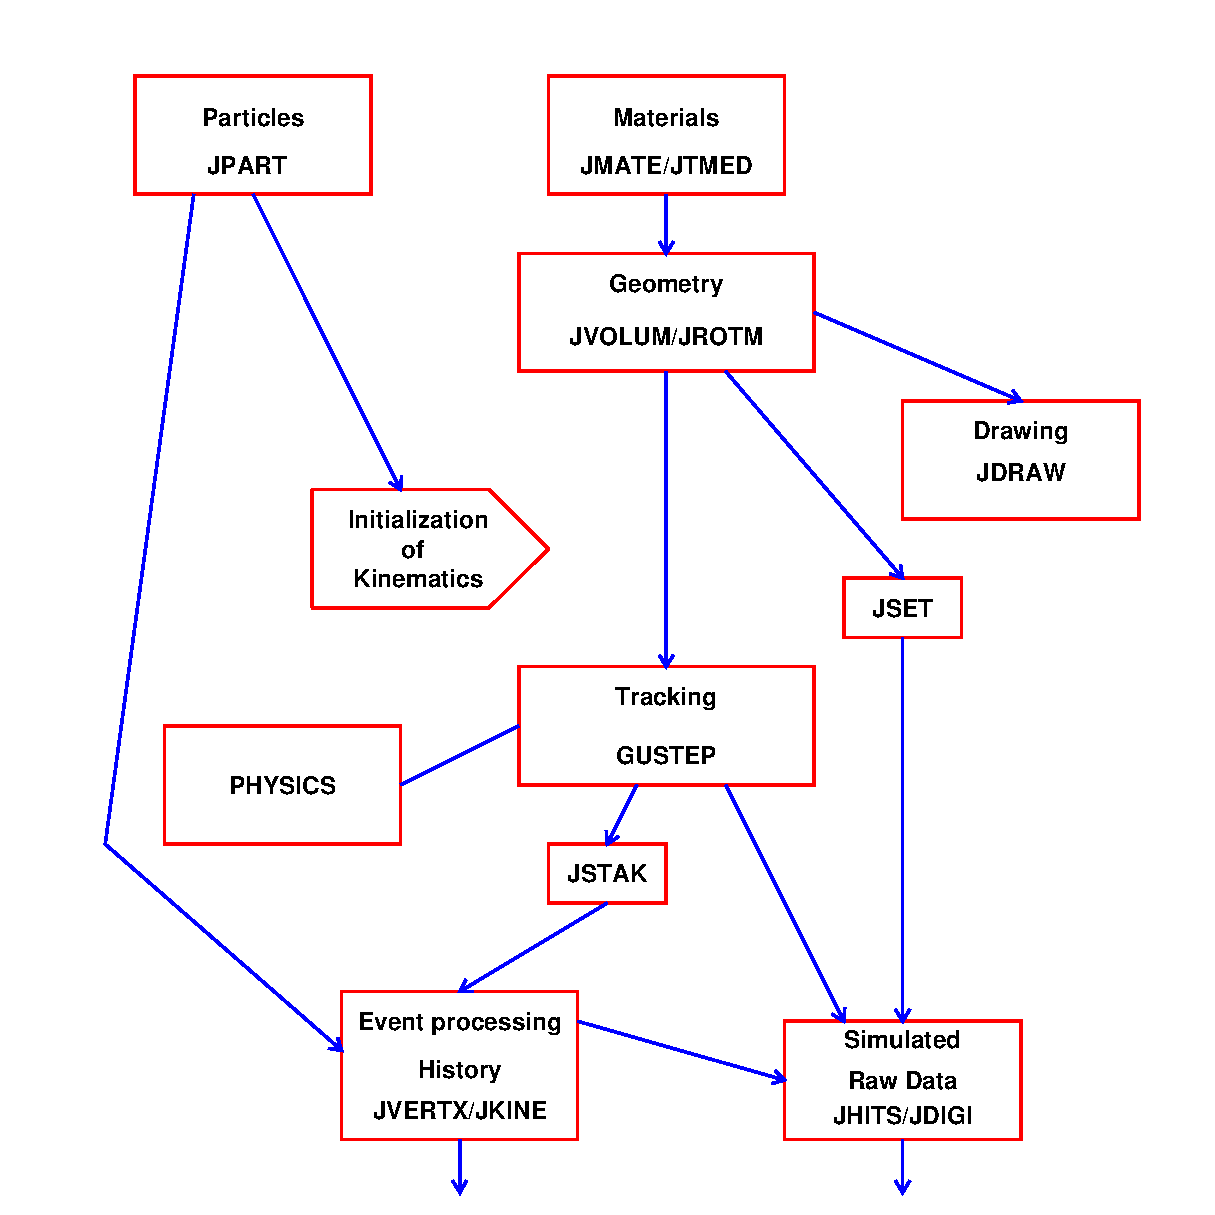
\epsfig{file=eps/base020-1.eps,width=12cm}
     \caption{Relation between {\tt GEANT} data structures}
     \label{fg:base020-1}
\end{figure}
\newpage

\section{Common blocks}
The communication between program segments of the {\tt GEANT} system
is assured by the contents of the data structures and by the definition
of {\it long range} variables in several common blocks.
In addition, within the program segments,
the subroutines communicate with each other through actual arguments
and through the common block variables. A detailed list of the 
user accessed common blocks is given in  {\tt [ZZZZ010]}. 
Their also the variables initialized in \Rind{GINIT} and the possibility
in overriding them through data records {\tt [BASE040]} or 
interactive commands {\tt [XINT]} are specified.
 
In most of the cases there is a correspondence between a
given data structure and a given common block where the current contents of
the banks are stored.
The labelled common blocks are accessible through Patchy/CMZ sequences
identified by the name of the {\tt COMMON}. They are defined in the Patch
\Rind {GCDES}.
 
{\bf Note:}
 
Unless otherwise specified, the long range variables are
initialised in \Rind{GINIT}. When non-zero, default values are
quoted between brackets. If the value may be modified
the keyword for the data record and for the interactive
command is also given in bold characters between brackets.
 

 
 

%%%%%%%%%%%%%%%%%%%%%%%%%%%%%%%%%%%%%%%%%%%%%%%%%%%%%%%%%%%%%%%%%%%
%                                                                 %
%  GEANT manual in LaTeX form                                     %
%                                                                 %
%  Version 1.00                                                   %
%                                                                 %
%  Last Mod.  9 June 1993 19:30  MG                               %
%                                                                 %
%%%%%%%%%%%%%%%%%%%%%%%%%%%%%%%%%%%%%%%%%%%%%%%%%%%%%%%%%%%%%%%%%%%
\Authors{F.Carminati}      \Origin{GEANT3}
\Version{Geant 3.12}\Routid{BASE030}
\Submitted{01.10.84}  \Revised{05.08.93}
\Makehead{Overview of COMMON Blocks}
\section{Introduction}
 
The communication between program segments of the GEANT3 system
is ensured by the contents of the data structures and by the definition
of `long range' variables in several common blocks.
In addition, within the program segments,
the subroutines communicate with each other through explicit arguments
and through the common block variables.
 
The data structures are described in separate papers. Here, the
main features of the common blocks used in GEANT3 are summarized,
with special mention of the variables initialized in \Rind{GINIT}
and of the possibility of overriding them through data records
{\tt [BASE040]} or interactive commands {\tt [XINT]}.
In most of the cases there is a correspondance between a
given data structure and a given common block where the current contents of
the banks are stored.
The labelled common blocks are accessible through Patchy sequences
identified by the name of the {\tt COMMON}. They are defined in the Patch
\Rind {GCDES}.
 
{\bf Note:}
 
Unless otherwise specified, the long range variables are
initialized in \Rind{GINIT}. When non-zero, default values are
quoted between brackets. If the value may be modified
the keyword for the data record and for the interactive
command is also given in bold characters between brackets.
 
\subsection{Dynamic memory}
 
The GEANT3 data structures are stored in the
common \FCind{/GCBANK/} accessible through the following Patchy sequence:
\FComm{GCBANK}{Dynamic core for the GEANT data structures}
\begin{verbatim}
      PARAMETER (KWBANK=69000,KWWORK=5200)
      COMMON/GCBANK/NZEBRA,GVERSN,ZVERSN,IXSTOR,IXDIV,IXCONS,FENDQ(16)
     +             ,LMAIN,LR1,WS(KWBANK)
      DIMENSION IQ(2),Q(2),LQ(8000),IWS(2)
      EQUIVALENCE (Q(1),IQ(1),LQ(9)),(LQ(1),LMAIN),(IWS(1),WS(1))
      EQUIVALENCE (JCG,JGSTAT)
      COMMON/GCLINK/JDIGI ,JDRAW ,JHEAD ,JHITS ,JKINE ,JMATE ,JPART
     +      ,JROTM ,JRUNG ,JSET  ,JSTAK ,JGSTAT,JTMED ,JTRACK,JVERTX
     +      ,JVOLUM,JXYZ  ,JGPAR ,JGPAR2,JSKLT
C
\end{verbatim}
The \FCind{/GCLINK/} variables are pointers to the GEANT3 data structures in
the \FCind{/GCBANK/} common.
They belong to a permanent area declared in \Rind{GZINIT}.
\subsection{Other labelled COMMON blocks}
\FComm{GCCUTS}{Tracking thresholds}
\begin{verbatim}
 COMMON/GCCUTS/CUTGAM,CUTELE,CUTNEU,CUTHAD,CUTMUO,BCUTE,BCUTM,
 +             DCUTE,DCUTM,PPCUTM,TOFMAX,GCUTS(5)
\end{verbatim}
\begin{DLtt}{MMMMMMMMMM}
\item[CUTGAM]    Kinetic energy cut threshold for gammas
({\tt 0.001, CUTS})
\item[CUTELE]    Kinetic energy cut threshold for electrons
({\tt 0.001, CUTS})
\item[CUTNEU]    Kinetic energy cut threshold for neutral hadrons
({\tt 0.01, CUTS})
\item[CUTHAD]    Kinetic energy cut threshold for charged hadrons
({\tt 0.01, CUTS})
\item[CUTMUO]    Kinetic energy cut threshold for muons
({\tt 0.01, CUTS})
\item[BCUTE]     Kinetic energy cut threshold for electron
                 Bremsstrahlung ({\tt CUTGAM, CUTS})
\item[BCUTM]    Kinetic energy cut threshold for muon Bremsstrahlung
({\tt CUTGAM, CUTS})
\item[DCUTE]   Kinetic energy cut threshold for electron delta rays
({\tt CUTELE, CUTS})
\item[DCUTM]  Kinetic energy cut threshold for muon or hadron delta rays
({\tt CUTELE, CUTS})
\item[PPCUTM] Total energy cut threshold for \Pep\Pem pair production by
              muon ({\tt 0.002, CUTS})
\item[TOFMAX]  Tracking cut threshold on time of flight integrated
from primary interaction time ({\tt $10^{10}$, CUTS})
\item[GCUTS]   For user applications   ({\tt CUTS})
\end{DLtt}
{\bf Note:}
The cuts {\tt BCUTE, BCUTM} and {\tt DCUTE, DCUTM} are given
the respective default values {\tt CUTGAM} and {\tt CUTELE}.
Experienced
users can make use of the facility offered (command {\tt CUTS})
to change {\tt BCUTE, DCUTE, BCUTM} and {\tt DCUTM}.
 
\FComm{GCDRAW}{Variables used by the drawing package}
\begin{verbatim}
      COMMON/GCDRAW/NUMNOD,MAXNOD,NUMND1,LEVVER,LEVHOR,MAXV,IPICK,
     + MLEVV,MLEVH,NWCUT,JNAM,JMOT,JXON,JBRO,JDUP,JSCA,JDVM,JPSM,
     + JNAM1,JMOT1,JXON1,JBRO1,JDUP1,JSCA1,JULEV,JVLEV,
     + LOOKTB(16),
     + GRMAT0(10),GTRAN0(3),IDRNUM,GSIN(41),GCOS(41),SINPSI,COSPSI,
     + GTHETA,GPHI,GPSI,GU0,GV0,GSCU,GSCV,NGVIEW,
     + ICUTFL,ICUT,CTHETA,CPHI,DCUT,NSURF,ISURF,
     + GZUA,GZVA,GZUB,GZVB,GZUC,GZVC,PLTRNX,PLTRNY,
     + LINATT,LINATP,ITXATT,ITHRZ,IPRJ,DPERS,ITR3D,IPKHIT,IOBJ,LINBUF,
     + MAXGU,MORGU,MAXGS,MORGS,MAXTU,MORTU,MAXTS,MORTS,
     + IGU,IGS,ITU,ITS,NKVIEW,IDVIEW,
     + NOPEN,IGMR,IPIONS,ITRKOP,IHIDEN,
     + DDUMMY(18)
C
\end{verbatim}
\begin{DLtt}{MMMMMMMMMM}
\item[NUMNOD] number of nodes in non-optimized tree
\item[MAXNOD] max. number of nodes of non-optimized tree.
({\tt MIN(NLEFT,16,200)}).
\item[NUMND1] number of nodes in optimized tree
\item[LEVVER] vertical level in the tree currently scanned by tree routines
\item[LEVHOR] horizontal node in the tree currently scanned by
tree routines
\item[MAXV] max vertical levels in the tree to be scanned by tree routines
\item[IPICK] node selected by \Rind{GDTREE}
\item[MLEVV] number of vertical levels in the last tree scanned
\item[MLEVH] number of horizontal nodes in the last tree scanned
\item[NWCUT] max. workspace allocated by cut routines, ({\tt 5000})
\item[JNAM-JVLEV]  pointers used by the tree routines
\item[LOOKTB] colour look-up table, ({\tt LOOKTB(I)=I,I=1,16})
\item[GRMAT0] rotation matrix saved by \Rind{GDRVOL}, ({\tt unitary matrix})
\item[GTRAN0] translation matrix saved by \Rind{GDRVOL}, ({\tt 0.,0.,0.})
\item[IDRNUM] flag for \Rind{GDRAW}, set to 1 when called by \Rind{GDRVOL},
({\bf 0})
\item[GSIN] sine table (at $9^{\circ}$ steps)
\item[GCOS] cosine table (at $9^{\circ}$ steps)
\item[SINPSI] {\tt SIN(GPSI*DEGRAD)}
\item[COSPSI] {\tt COS(GPSI DEGRAD)}
\item[GTHETA] $\theta$ angle of the parallel projection of 3-dimensional
images on the screen (${\tt 45^{\circ}}$)
\item[GPHI]  $\phi$ angle of the parallel projection of 3-dimensional
images on the screen (${\tt 135^{\circ}}$)
\item[GPSI]  $\psi$ angle of rotation of the image on the screen
(${\tt 0^{\circ}}$)
\item[GU0]  U position (X in screen coordinates) of the origin of the drawing
screen in screen units ({\tt 10.})
\item[GV0]  V position (Y in screen coordinates) of the origin of the drawing
screen in screen units ({\tt 10.})
\item[GSCU]   scale factor for the U screen coordinate  ({\tt 0.015})
\item[GSCV]   scale factor for the V screen coordinate ({\tt 0.015})
\item[NGVIEW] flag informing \Rind{GDFR3D} and \Rind{GD3D3D} if
the view point has changed  ({\tt 0})
\item[ICUTFL] flag informing \Rind{GDRAW} if it was called by
{\it cut} routines
\item[ICUT] axis along which the cut is performed (1, 2 or 3, 0 if no cut)
\item[CTHETA] $\theta$ angle of cut supplied to \Rind{GDRAWX} (used by
\Rind{GDCUT})
\item[CPHI] $\phi$ angle of cut supplied to \Rind{GDRAWX} (used by
\Rind{GDCUT})
\item[DCUT] coordinate value (along axis {\tt ICUT)} at which the cut is
performed
\item[NSURF] number of surfaces stored in {\tt SURF}
\item[ISURF] pointer for array {\tt SURF}
\item[GZUA] zoom parameter (horizontal scale factor)  ({\tt 1.})
\item[GZVA] zoom parameter (vertical scale factor)  ({\tt 1.})
\item[GZUB] zoom parameter  ({\tt 0.})
\item[GZVB] zoom parameter  ({\tt 0.})
\item[GZUC] zoom parameter  ({\tt 0.})
\item[GZVC] zoom parameter  ({\tt 0.})
\item[PLTRNX] screen and plotter X range, {\tt PLTRNX} $\times$
{\tt PLTRNY} cm. ({\tt 20.})
\item[PLTRNY] screen and plotter Y range, {\tt PLTRNX} $\times$
{\tt PLTRNY} cm. ({\tt 20.})
\item[LINATT] current line attributes ({\tt colour=1, width=1, style=1,
fill=1})
\item[LINATP] permanent line attributes  ({\tt LINATT)}
\item[ITXATT] current text attributes  ({\tt colour = 1, width = 1})
\item[ITHRZ] string containing the status of {\tt THRZ} option of
            \Rind{GDOPT}  ({\tt 'OFF '})
\item[IPRJ] string containing the status of {\tt PROJ} option of
            \Rind{GDOPT}  ({\tt 'PARA'})
\item[DPERS] distance of the view point from
the origin (used with perspective) ({\tt 1000.})
\item[ITR3D]track being scanned (used together with {\tt THRZ} option)
\item[IPKHIT]flag for \Rind{GPHITS}, if
$>0$ then print only hit number, ({\tt 0})
\item[IOBJ]type of the object being drawn (detector, track, hit, etc.)
({\tt 0})
\item[LINBUF]flag informing \Rind{GDRAWV} if line buffering is wanted or
not ({\tt 0})
\item[MAXGU]current physical number of words for graphic unit banks
\item[MORGU]number of words to be pushed in graphic unit banks
\item[MAXGS]current physical number of words for graphic segment banks
\item[MORGS]number of words to be pushed in graphic segment banks
\item[MAXTU]current physical number of words for text unit banks
\item[MORTU]number of words to be pushed in text unit banks
\item[MAXTS]current physical number of words for text segment banks
\item[MORTS]number of words to be pushed in text segment banks
\item[IGU]pointer to current graphic unit bank
\item[IGS]pointer to current graphic segment bank
\item[ITU]pointer to current text unit bank
\item[ITS]pointer to current text segment bank
\item[NKVIEW]number of view data banks ({\tt 0})
\item[IGVIEW]current view bank number or 0 for screen ({\tt 0})
\item[NOPEN]unused ({\tt 0})
\item[IGMR]flag informing if {\tt APOLLO-GMR} is being used ({\tt 0})
\item[IPIONS]unused ({\tt 0})
\item[ITRKOP]string containing the status of {\tt TRAK} option of
\Rind{GDOPT} ({\tt 'LINE'})
\item[DDUMMY]array of dummy words
\end{DLtt}
\FComm{GCFLAG}{Flags and variables to control the run}
\begin{verbatim}
      COMMON/GCFLAG/IDEBUG,IDEMIN,IDEMAX,ITEST,IDRUN,IDEVT,IEORUN
     +        ,IEOTRI,IEVENT,ISWIT(10),IFINIT(20),NEVENT,NRNDM(2)
C
\end{verbatim}
\begin{DLtt}{MMMMMMMMMM}
\item[IDEBUG]Flag set internally to 1 to activate debug
output if {\tt IEVENT} (below)
\item[IDEMIN]     is greater or equal to {\tt IDEMIN} ({\tt DEBU})
\item[IDEMAX]     and less or equal to {\tt IDEMAX}   ({\tt DEBU})
\item[ITEST]Flag to request printing of {\tt IEVENT, IDEVT} and {\tt
NRNDM} (below) every {\tt ITEST} events ({\tt DEBU})
\item[IDRUN]Current user run number   ({\tt 1, RUNG})
\item[IDEVT]Current user event number  ({\tt 1, RUNG})
\item[IEORUN]Flag to terminate run if non-zero
\item[IEOTRI]Flag to abort current event if non-zero
\item[IEVENT]Current event sequence number ({\tt 1})
\item[ISWIT]Flags reserved for user in relation to debug ({\tt 0, SWIT})
\item[IFINIT]Flags used for initialisation
\item[NEVENT]Number of events to be processed  ({\tt 10000000, TRIG})
\item[NRNDM]Initial seeds for the random number generator. If
{\tt NRNDM(2)=0} the sequence number {\tt NRNDM(1)} is taken from a
predefined set of 215 indipendent sequences. Otherwise the random
number generator is initialised with the two seeds {\tt NRNDM(1), NRNDM(2)}.
({\tt 9876, 54321})
\end{DLtt}
\FComm{GCGOBJ}{CG package variables}
\begin{verbatim}
      PARAMETER (NTRCG=1)
      PARAMETER (NWB=207,NWREV=100,NWS=1500)
      PARAMETER (C2TOC1=7.7, C3TOC1=2.,TVLIM=1296.)
      COMMON /GCGOBJ/IST,IFCG,ILCG,NTCUR,NFILT,NTNEX,KCGST
     +             ,NCGVOL,IVFUN,IVCLOS,IFACST,NCLAS1,NCLAS2,NCLAS3
      COMMON /CGBLIM/IHOLE,CGXMIN,CGXMAX,CGYMIN,CGYMAX,CGZMIN,CGZMAX
C
\end{verbatim}
\begin{DLtt}{MMMMMMMMMM}
\item[NTRCG]
\item[NWB]
\item[NWREV]
\item[NWS]
\item[C2TOC1]
\item[C3TOC1]
\item[TVLIM]
\item[IST]
\item[IFCG]
\item[ILCG]
\item[NTCUR]
\item[NFILT]
\item[NTNEX]
\item[KCGST]
\item[NCGVOL]
\item[IVFUN]
\item[IVCLOS]
\item[IFACST]
\item[NCLAS1]
\item[NCLAS2]
\item[NCLAS3]
\item[IHOLE]
\item[CGXMIN]
\item[CGXMAX]
\item[CGYMIN]
\item[CGYMAX]
\item[CGZMIN]
\item[CGZMAX]
\end{DLtt}
\FComm{GCHILN}{Temporary link area for the CG package}
\begin{verbatim}
      COMMON/GCHILN/LARECG(2), JCGOBJ, JCGCOL, JCOUNT, JCLIPS,
     +              ICLIP1, ICLIP2
*
\end{verbatim}
\FComm{GCJLOC}{JMATE substructure pointers for current material}
\begin{verbatim}
      COMMON/GCJLOC/NJLOC(2),JTM,JMA,JLOSS,JPROB,JMIXT,JPHOT,JANNI
     +                  ,JCOMP,JBREM,JPAIR,JDRAY,JPFIS,JMUNU,JRAYL
     +                  ,JMULOF,JCOEF,JRANG
C
\end{verbatim}
 
See {\tt [CONS199]}.
\FComm{GCJUMP}{Pointers for the jump package}
\begin{verbatim}
      PARAMETER    (MAXJMP=30)
      COMMON/GCJUMP/JUDCAY, JUDIGI, JUDTIM, JUFLD , JUHADR, JUIGET,
     +              JUINME, JUINTI, JUKINE, JUNEAR, JUOUT , JUPHAD,
     +              JUSKIP, JUSTEP, JUSWIM, JUTRAK, JUTREV, JUVIEW,
     +              JUPARA
      DIMENSION     JMPADR(MAXJMP)
      EQUIVALENCE  (JMPADR(1), JUDCAY)
*
\end{verbatim}
\FComm{GCKINE}{Kinematics of current track}
 
\begin{verbatim}
      COMMON/GCKINE/IKINE,PKINE(10),ITRA,ISTAK,IVERT,IPART,ITRTYP
     +      ,NAPART(5),AMASS,CHARGE,TLIFE,VERT(3),PVERT(4),IPAOLD
C
\end{verbatim}
\begin{DLtt}{MMMMMMMMMM}
\item[IKINE]  user integer word  ({\tt 0, KINE})
\item[PKINE]  user array of real   ({\tt 0, KINE})
\item[ITRA]   Current track number
\item[ISTAK]Current stack track number
\item[IVERT]Current vertex number
\item[IPART]Current particle number
\item[ITRTYP]Current particle tracking type
\item[NAPART] Name of current particle (ASCII codes stored in an integer
array, 4 characthers per word)
\item[AMASS]  Mass of current particle
\item[CHARGE]Charge of current particle
\item[TLIFE]Average life time of current particle
\item[VERT]Coordinates of origin vertex for current track
\item[PVERT]Track kinematics at origin vertex ({\tt PVERT(4)} not used)
\item[IPAOLD]Particle number of the previous track.
\end{DLtt}
\FComm{GCKMAX}{Size of the \FCind{/GCKING/} stack}
\begin{verbatim}
      INTEGER MXGKIN
      PARAMETER (MXGKIN=100)
\end{verbatim}
\FComm{GCMUTR}{Auxiliary variables for the CG package}
\begin{verbatim}
      PARAMETER (MULTRA=50)
      CHARACTER*4 GNASH, GNNVV, GNVNV
      COMMON/GCMUTR/NCVOLS,KSHIFT,NSHIFT,ICUBE,NAIN,JJJ,
     +              NIET,IOLDSU,IVOOLD,IWPOIN,IHPOIN,IVECVO(100),
     +              PORGX,PORGY,PORGZ,POX(15),POY(15),POZ(15),GBOOM,
     +              PORMIR(18),PORMAR(18),IPORNT,
     +              ICGP,CLIPMI(6),CLIPMA(6),
     +              ABCD(4),BMIN(6),BMAX(6),CGB(16000),CGB1(16000),
     +              GXMIN(MULTRA),GXMAX(MULTRA),GYMIN(MULTRA),
     +              GYMAX(MULTRA),GZMIN(MULTRA),GZMAX(MULTRA),
     +              GXXXX(MULTRA),GYYYY(MULTRA),GZZZZ(MULTRA)
*
      COMMON/GCMUTC/   GNASH(MULTRA),GNNVV(MULTRA),GNVNV(MULTRA)
*
\end{verbatim}
\FComm{GCKING}{Kinematics of generated secondaries}
\begin{verbatim}
      COMMON/GCKING/KCASE,NGKINE,GKIN(5,MXGKIN),
     +                           TOFD(MXGKIN),IFLGK(MXGKIN)
C
      PARAMETER (MXPHOT=1000)
      COMMON/GCKIN2/NGPHOT,XPHOT(11,MXPHOT)
C
\end{verbatim}
\begin{DLtt}{MMMMMMMMMM}
\item[KCASE] Mechanism which has generated the secondary particles
\item[NGKINE]Number of generated secondaries
\item[GKIN(1,I)]x component of momentum of ${\rm I}^{th}$ particle
\item[GKIN(2,I)]y component of momentum
\item[GKIN(3,I)]z component of momentum
\item[GKIN(4,I)]Total energy
\item[GKIN(5,I)]Particle code
\item[TOFD(I)]Time offset with respect to current time of flight
\item[IFLGK(I)]Flag controlling the handling of track by {\tt GSKING/GSSTAK}
\begin{DLtt}{MMMMM}
\item[$<0$=]particle is stored in  the temporary stack {\tt JSTAK} and in
the data structure {\tt JKINE} attached to vertex {\tt -IFLGK(I)}
\item[0 =]({\bf D}) particle is stored in the temporary stack {\tt JSTAK}
for further tracking
\item[1 =] like {\tt 0} but
particle is stored in {\tt JVERTX/JKINE} structure as well
\item[2 =] entry in {\tt JKINE} already exists for this track
\end{DLtt}
\item[NGPHOT] number of \v{C}erenkov photons generated in the current
step
\item[XPHOT(1,I)] x position of the ${\rm I}^{th}$ photon
\item[XPHOT(2,I)] y position
\item[XPHOT(3,I)] z position
\item[XPHOT(4,I)] x component of momentum
\item[XPHOT(5,I)] y component of momentum
\item[XPHOT(6,I)] z component of momentum
\item[XPHOT(7,I)] momentum of the photon
\item[XPHOT(8,I)] x component of the polarisation vector
\item[XPHOT(9,I)] y component of the polarisation vector
\item[XPHOT(10,I)] z component of the polarisation vector
\item[XPHOT(11,I)] time of flight in seconds of the photon
\end{DLtt}
\FComm{GCLINK}{See \FCind{/GCBANK/} above}
\FComm{GCLIST}{Various system and user lists}
\begin{verbatim}
      COMMON/GCLIST/NHSTA,NGET ,NSAVE,NSETS,NPRIN,NGEOM,NVIEW,NPLOT
     +       ,NSTAT,LHSTA(20),LGET (20),LSAVE(20),LSETS(20),LPRIN(20)
     +             ,LGEOM(20),LVIEW(20),LPLOT(20),LSTAT(20)
C
\end{verbatim}
\begin{DLtt}{MMMMMMMMMM}
\item[NHSTA] Number of histograms declared on data record {\tt HSTA }
\item[NGET] Number of data structures declared on data record {\tt GET}
\item[NSAVE]Number of data structures declared on data record {\tt SAVE}
\item[NSETS]Number of items described on data record {\tt SETS}
\item[NPRIN]Number of items described on data record {\tt PRIN}
\item[NGEOM]Number of items described on data record {\tt GEOM}
\item[NVIEW]Number of items described on data record {\tt VIEW}
\item[NPLOT]Number of items described on data record {\tt PLOT}
\item[NSTAT]Number of items described on data record {\tt STAT}. Obsolete.
\item[LHSTA,\ldots LSTAT]Corresponding user lists of items
({\tt HSTA,\ldots,STAT})
\end{DLtt}
{\tt LSTAT(1)} is reserved by the system for volume statistics.
\FComm{GCMATE}{Parameters of current material}
\begin{verbatim}
      COMMON/GCMATE/NMAT,NAMATE(5),A,Z,DENS,RADL,ABSL
C
\end{verbatim}
\begin{DLtt}{MMMMMMMMMM}
\item[NMAT]  Current material number
\item[NAMATE]Name of current material (ASCII codes stored in an integer
array, 4 characthers per word)
\item[A]Atomic weight of current material
\item[Z]Atomic number of current material
\item[DENS]Density of current material in ${\rm g \: \: cm^{-3}}$
\item[RADL]Radiation length of current material
\item[ABSL]Absorption length of current material
\end{DLtt}
\FComm{GCMULO}{Energy binning and multiple scattering}
 
Precomputed quantities for multiple scattering and energy binning for
{\tt JMATE} banks. See also {\tt [CONS199]} for the energy binning and
{\tt [PHYS325]} for a description of the variables {\tt OMCMOL} and
{\tt CHCMOL}.
\begin{verbatim}
      COMMON/GCMULO/SINMUL(101),COSMUL(101),SQRMUL(101),OMCMOL,CHCMOL
     +  ,EKMIN,EKMAX,NEKBIN,NEK1,EKINV,GEKA,GEKB,EKBIN(200),ELOW(200)
\end{verbatim}
\begin{DLtt}{MMMMMMMMMM}
\item[SINMUL]  Not used any more
\item[COSMUL]  Not used any more
\item[SQRMUL]  Not used any more
\item[OMCMOL]  Constant $\Omega_0$ of the Moli\'ere theory
\item[CHCMOL]  Constant of the Moli\'ere theory
\item[EKMIN]   Lower edge of the energy range of the tabulated cross
sections ({\tt $10^{-5}$, ERAN})
\item[EKMAX]   Upper edge of the energy range of the tabulated cross
sections ({\tt $10^{4}$, ERAN})
\item[NEKBIN]    Number of energy bins to be used ({\tt 90, ERAN})
\item[NEK1]    {\tt NEKBIN+1}
\item[EKINV]   $1/ \left ( \log_{10}({\tt EKMAX})-
\log_{10}({\tt EKMIN}) \right )$
\item[GEKA]    {\tt NEKBIN*EKINV}
\item[GEKB]    {\tt 1-GEKA*EKBIN(1)}
\item[EKBIN]   $\log \left ( {\tt ELOW} \right ) $
\item[ELOW]    Low edges of the energy bins
\end{DLtt}
\FComm{GCMZFO}{I/O descriptors of GEANT banks}
\begin{verbatim}
      COMMON/GCMZFO/IOMATE,IOPART,IOTMED,IOSEJD,IOSJDD,IOSJDH,IOSTAK
     +             ,IOMZFO(13)
C
\end{verbatim}
\FComm{GCNUM}{Current number for various items}
\begin{verbatim}
      COMMON/GCNUM/NMATE ,NVOLUM,NROTM,NTMED,NTMULT,NTRACK,NPART
     +            ,NSTMAX,NVERTX,NHEAD,NBIT
      COMMON /GCNUMX/ NALIVE,NTMSTO
C
\end{verbatim}
\begin{DLtt}{MMMMMMMMMM}
\item[NMATE]      Number of Materials
\item[NVOLUM]     Number of Volumes
\item[NROTM]      Number of Rotation matrices
\item[NTMED]      Number of Tracking media
\item[NTMULT]     Number of tracks processed in current event
                 (including secondaries), reset to 0 for each event
\item[NTRACK]    Number of Tracks in {\tt JKINE} bank for current event
\item[NPART]     Maximum particle code
\item[NSTMAX]    Maximum number of tracks in stack {\tt JSTAK}
                 for current event, reset to 0 for each event
\item[NVERTX]   Number of Vertices in {\tt JVERTX} mother bank for current event
\item[NHEAD]    Number of data words in the {\tt JHEAD} bank ({\tt 10})
\item[NBIT]    Number of bits per word (initialized in \Rind{GINIT}
               via {\tt ZEBRA})
\end{DLtt}
\begin{DLtt}{MMMMMMMMMM}
\item[NALIVE]Number of particles to be tracked in the parallel tracking stack
(see {\tt [TRAK???]}
\item[NTMSTO]Total number of tracks tracked in the current event so far. Same
as {\tt NTMULT} in \FCind{/GCTRAK/}.
\end{DLtt}
\FComm{GCOMIS}{Variables for the COMIS package}
\begin{verbatim}
      COMMON/GCOMIS/ICOMIS,JUINIT,JUGEOM,JUKINE,JUSTEP,JUOUT,JULAST
*
\end{verbatim}
\FComm{GCONST}{Basic constants}
\begin{verbatim}
      COMMON/GCONST/PI,TWOPI ,PIBY2,DEGRAD,RADDEG,CLIGHT ,BIG,EMASS
      COMMON/GCONSX/EMMU,PMASS,AVO
C
\end{verbatim}
\begin{DLtt}{MMMMMMMMMM}
\item[PI]         $\pi$ ({\tt ACOS(-1)})
\item[TWOPI]      $2\pi$
\item[PIBY2]      $\pi/2$
\item[DEGRAD]    Degree to radian conversion factor ($\pi/180$)
\item[RADDEG]    Radian to degree conversion factor ($180/\pi$)
\item[CLIGHT]    Light velocity ($2.99792458 \times 10^{10}
\: cm \: sec^{-1}$)
\item[BIG]       Arbitrary large number ($10^{10}$)
\item[EMASS]     Electron mass ($0.5110034 \times 10^{-3} \: GeV$)
\item[EMMU]      Muon mass ($0.105659 \: GeV$)
\item[PMASS]     Proton mass ($0.93828 \: GeV$)
\item[AVO]       Avogadro's number $\times 10^{23}$ ($0.6022045$)
\end{DLtt}
 
\FComm{GCOPTI}{Control of Geometry optimisation}
\begin{verbatim}
      COMMON/GCOPTI/ IOPTIM
C
\end{verbatim}
\begin{DLtt}{MMMMMMMMMM}
\item[IOPTIM]Optimization flag
\begin{DLtt}{MMMMM}
\item[-1 =] No optimisation at all. \Rind{GSORD} calls disabled
\item[~0 =] No optimisation. Only user calls to \Rind{GSORD} kept
\item[~1 =] All non-\Rind{GSORD}ered volumes are ordered along the best axis
\item[~2 =] All volumes are ordered along the best axis
\end{DLtt}
\end{DLtt}
\FComm{GCPARA}{Control of parametrized energy deposition}
\begin{verbatim}
      PARAMETER (LSTACK = 5000)
      LOGICAL    SYMPHI, SYMTEU, SYMTED
C
      COMMON    /GCPARA/
     +                   JJLOST, EPSMAX, JJWORK,
     +                   IFOUNP, IFOUNT, IFNPOT,
     +                   SYMPHI, SYMTEU, SYMTED
C
\end{verbatim}
\begin{DLtt}{MMMMMMMMMM}
\item[LSTACK] Dimension of the Energy ray stack
\item[JJLOST] Number of Energy rays lost in each tracking step
\item[EPSMAX] Maximum number of radiation
lengths that an Energy ray can travel
\item[JJWORK] Actual size of the Energy ray stack
\item[IFOUNP] Number of Energy rays that change cell in $\phi$
direction
\item[IFOUNT] Number of Energy rays that change cell in $\theta$
direction
\item[IFNPOT] Number of Energy rays that change cell either in $\phi$
or in $\theta$
\item[SYMPHI] {\tt .TRUE.} if ${\tt PHIMAX-PHIMIN = 360^{\circ}}$
\item[SYMTEU] {\tt .TRUE.} if ${\tt TETMIN = 0^{\circ}}$
\item[SYMTED] {\tt .TRUE.} if ${\tt TETMAX = 180^{\circ}}$
\end{DLtt}
\FComm{GCPARM}{Control of parametrization}
\begin{verbatim}
      COMMON/GCPARM/IPARAM,PCUTGA,PCUTEL,PCUTNE,PCUTHA,PCUTMU
     +             ,NSPARA,MPSTAK,NPGENE
      REAL PACUTS(5)
      EQUIVALENCE (PACUTS(1),PCUTGA)
      PARAMETER (NWPPAR=14)
      PARAMETER (NWERAY=40)
C
\end{verbatim}
\begin{DLtt}{MMMMMMMMMM}
\item[IPARAM]Parametrization flag ({\tt 0, PCUT})
\begin{DLtt}{MMMMM}
\item[0 =]parametrization is not in effect, normal tracking will be used
\item[1 =]parametrization is in effect
\end{DLtt}
\item[PCUTGA]Parametrization threshold for photons ({\tt 0.,  PCUT})
\item[PCUTEL]Parametrization threshold for electrons and positrons
({\tt 0.,  PCUT})
\item[PCUTNE]Parametrization threshold for neutral hadrons
({\tt 0., PCUT})
\item[PCUTHA]Parametrization threshold for charged hadrons
({\tt 0., PCUT})
\item[PCUTMU]Parametrization threshold for muons
({\tt 0.,  PCUT})
\item[NSPARA] not used
\item[MPSTAK] Optimum size of the Energy ray stack ({\tt 2000})
\item[NPGENE] Number of Energy rays generated per primary particle
({\tt 20})
\item[NWPPAR] Number of words stored for each track to be parametrized
\item[NWERAY] Number of words stored for each Energy-ray
\end{DLtt}
\FComm{GCPHYS}{Control of physics processes}
\begin{verbatim}
   COMMON/GCPHYS/IPAIR, SPAIR, SLPAIR,ZINTPA,STEPPA
  +             ,ICOMP, SCOMP, SLCOMP,ZINTCO,STEPCO
  +             ,IPHOT, SPHOT, SLPHOT,ZINTPH,STEPPH
  +             ,IPFIS, SPFIS, SLPFIS,ZINTPF,STEPPF
  +             ,IDRAY, SDRAY, SLDRAY,ZINTDR,STEPDR
  +             ,IANNI, SANNI, SLANNI,ZINTAN,STEPAN
  +             ,IBREM, SBREM, SLBREM,ZINTBR,STEPBR
  +             ,IHADR, SHADR, SLHADR,ZINTHA,STEPHA
  +             ,IMUNU, SMUNU, SLMUNU,ZINTMU,STEPMU
  +             ,IDCAY, SDCAY, SLIFE ,SUMLIF,DPHYS1
  +             ,ILOSS, SLOSS, SOLOSS,STLOSS,DPHYS2
  +             ,IMULS, SMULS, SOMULS,STMULS,DPHYS3
 
\end{verbatim}
\begin{DLtt}{MMMMMMMMMM}
\item[IPAIR] Control variable for the \Pem/\Pep pair production process.
\item[SPAIR] Distance to the next pair production in the current material.
\item[SLPAIR] Distance travelled by the $\gamma$ when pair production occurs.
\item[ZINTPA] Number of interaction lengths to the next pair production.
\item[STEPPA] Interaction length for pair production for the current material
and energy.
\item[ICOMP] Control variable for the Compton scattering process.
\item[SCOMP] Distance to the next Compton scattering in the current material.
\item[SLCOMP] Distance travelled by the $\gamma$ when Compton scattering occurs.
\item[ZINTCO] Number of interaction lengths to the next Compton scattering.
\item[STEPCO] Interaction length for Compton scattering for the current material
and energy.
\item[IPHOT] Control variable for the photoelectric effect process.
\item[SPHOT] Distance to the next photoelectric effect in the current material.
\item[SLPHOT] Distance travelled by the $\gamma$ when photoelectric effect occurs.
\item[ZINTPH] Number of interaction lengths to the next photoelectric effect.
\item[STEPPH] Interaction length for photoelectric effect for the current material
and energy.
\item[IPFIS] Control variable for the $\gamma$-induced nuclear fission process.
\item[SPFIS] Distance to the next $\gamma$-induced nuclear fission in the current 
material.
\item[SLPFIS] Distance travelled by the $\gamma$ when $\gamma$-induced nuclear 
fission occurs.
\item[ZINTPF] Number of interaction lengths to the next $\gamma$-induced nuclear 
fission.
\item[STEPPF] Interaction length for $\gamma$-induced nuclear fission for the 
current material and energy.
\item[IDRAY] Control variable for the $\delta$-ray production process.
\item[SDRAY] Distance to the next $\delta$-ray production in the current material.
\item[SLDRAY] Distance travelled by the particle when $\delta$-ray production 
occurs.
\item[ZINTDR] Number of interaction lengths to the next $\delta$-ray production.
\item[STEPDR] Interaction length for $\delta$-ray production for the current 
material and energy.
\item[IANNI] Control variable for the positron annichilation process.
\item[SANNI] Distance to the next positron annichilation in the current material.
\item[SLANNI] Distance travelled by the positron when positron annichilation 
occurs.
\item[ZINTAN] Number of interaction lengths to the next positron annichilation.
\item[STEPAN] Interaction length for positron annichilation for the current 
material and energy.
\item[IBREM] Control variable for the Bremstrahlung process.
\item[SBREM] Distance to the next Bremstrahlung in the current material.
\item[SLBREM] Distance travelled by the particle when Bremstrahlung occurs.
\item[ZINTBR] Number of interaction lengths to the next Bremstrahlung.
\item[STEPBR] Interaction length for Bremstrahlung for the current material
and energy.
\item[IHADR] Control variable for the hadronic interaction process.
\item[SHADR] Distance to the next hadronic interaction in the current material.
\item[SLHADR] Distance travelled by the particle when hadronic interaction occurs.
\item[ZINTHA] Number of interaction lengths to the next hadronic interaction.
\item[STEPHA] Interaction length for hadronic interaction for the current material
and energy.
\item[IMUNU] Control variable for the $\mu$ nuclear interaction process.
\item[SMUNU] Distance to the next $\mu$ nuclear interaction in the current 
material.
\item[SLMUNU] Distance travelled by the $\mu$ when $\mu$ nuclear interaction 
occurs.
\item[ZINTMU] Number of interaction lengths to the next $\mu$ nuclear interaction.
\item[STEPMU] Interaction length for $\mu$ nuclear interaction for the current 
material and energy.
\item[IDCAY] Control variable for the decay in flight process.
\item[SDCAY] Distance to the next decay in flight in the current material.
\item[SLIFE] Distance travelled by the particle when decay in flight occurs.
\item[SUMLIF] Time to the next interaction point in $ct$ units.
\item[DPHYS1] Not used.
and energy.
\item[ILOSS] Control variable for the energy loss process.
\item[SLOSS] Step limitation due to the energy loss process.
\item[SOLOSS] Not used.
\item[STLOSS] Not used. Set equal to {\tt STEP} for backward compatibility.
\item[DPHYS2] Not used.
\item[IMULS] Control variable for the energy loss process.
\item[SMULS] Maximum step allowed by the multiple scattering simulation.
\item[SOMULS] Not used.
\item[STMULS] Not used. Set equal to step for backward compatibility.
\item[DPHYS3] Not used.
\end{DLtt}
For more details on {\tt IDRAY} and {\tt ILOSS} see {\tt [BASE040]}.
For all other variables see {\tt [PHYS010]}.
\FComm{GCPOLY}{Internal flags for polygon and polycone shapes}
\begin{verbatim}
      COMMON/GCPOLY/IZSEC,IPSEC
C
\end{verbatim}
\begin{DLtt}{MMMMMMMMMM}
\item[IZSEC]    Z  section number
\item[IPSEC]    $\phi$ sector number
\end{DLtt}
\FComm{GCPUSH}{Initial and incremental size of some mother banks}
\begin{verbatim}
      COMMON/GCPUSH/NCVERT,NCKINE,NCJXYZ,NPVERT,NPKINE,NPJXYZ
C
\end{verbatim}
\begin{DLtt}{MMMMMMMMMM}
\item[NCVERT] Initial size of mother bank {\tt JVERTX } ({\tt 5})
\item[NCKINE] Initial size of mother bank {\tt JKINE}  ({\tt 50})
\item[NCJXYZ] Initial size of mother bank {\tt JXYZ}  ({\tt 50})
\item[NPVERT] Increment for size of mother bank {\tt JVERTX}  ({\tt 5})
\item[NPKINE] Increment for size of mother bank {\tt JKINE}  ({\tt 10})
\item[NPJXYZ] Increment for size of mother bank {\tt JXYZ}  ({\tt 10})
\end{DLtt}
\FComm{GCRZ}{Direct access files control variables}
\begin{verbatim}
      COMMON/GCRZ1/NRECRZ,NRGET,NRSAVE,LRGET(20),LRSAVE(20)
      COMMON/GCRZ2/RZTAGS
      CHARACTER*8 RZTAGS(4)
C
\end{verbatim}
\begin{DLtt}{MMMMMMMMMM}
\item[NRECRZ] Record size (argument of {\tt RZMAKE})
\item[NRGET]  Number of data structures declared on data card {\tt RGET}
\item[NRSAVE] Number of data structures declared on data card {\tt RSAV}
\item[LRGET,LRSAVE] Corresponding user lists of items
\item[RZTAGS]Key names (argument of {\tt RZMAKE})
\end{DLtt}
\FComm{GCSCAL}{Scan geometry ZEBRA pointers}
\begin{verbatim}
      PARAMETER(MXSLNK=100)
      COMMON/GCSCAL/ ISLINK(MXSLNK)
      EQUIVALENCE (LSLAST,ISLINK(MXSLNK))
      EQUIVALENCE (LSCAN ,ISLINK(1)),(LSTEMP,ISLINK(2))
      EQUIVALENCE (LSPARA,ISLINK(3)),(LSERAY,ISLINK(4))
*
\end{verbatim}
\FComm{GCSCAN}{Scan geometry control parameters}
\begin{verbatim}
      PARAMETER (MSLIST=32,MAXMDT=3)
      COMMON/GCSCAN/SCANFL,NPHI,PHIMIN,PHIMAX,NTETA,TETMIN,TETMAX,
     +              MODTET,IPHIMI,IPHIMA,IPHI1,IPHIL,NSLMAX,
     +              NSLIST,ISLIST(MSLIST),VSCAN(3),FACTX0,FACTL,
     +              FACTR,IPHI,ITETA,ISCUR,SX0,SABS,TETMID(MAXMDT),
     +              TETMAD(MAXMDT)
     +             ,SX0S,SX0T,SABSS,SABST,FACTSF
     +             ,DLTPHI,DLTETA,DPHIM1,DTETM1
     +             ,FCX0M1,FCLLM1,FCRRM1
      LOGICAL SCANFL
      COMMON/GCSCAC/SFIN,SFOUT
      CHARACTER*80 SFIN,SFOUT
*
\end{verbatim}
\begin{DLtt}{MMMMMMMMMM}
\item[MSLIST] Dimension of {\tt ISLIST} array ({\tt 32})
\item[MAXMDT] Number of $\theta$ division types ({\tt 3})
\item[SCANFL] SCAN flag ({\tt .FALSE., SCAN, STURN})
\begin{DLtt}{MMMMMMMMMM}
\item[.TRUE.]creation of {\tt SCAN} geometry, geantinos will be tracked
\item[.FALSE.]normal tracking
\end{DLtt}
\item[NPHI] Number of $\phi$ divisions ({\tt 90, SCAN}, {\tt PHI})
\item[PHIMIN] Minimum $\phi$ in degrees (${\tt 0^{\circ}}$,
{\tt SCAN}, {\tt PHI})
\item[PHIMAX] Maximum $\phi$ in degrees (${\tt 360^{\circ}}$,
{\tt SCAN}, {\tt PHI})
\item[NTETA] Number of $\theta$ divisions ({\tt 90}, {\tt SCAN},
{\tt TETA})
\item[TETMIN] Minimum value of $\theta$
(${\tt 0^{\circ}}$, {\tt SCAN}, {\tt TETA})
\item[TETMAX] Maximum value of $\theta$ (18{\tt 0.,  SCAN}, {\tt $\theta$})
\item[MODTET] Type of $\theta$ division (1, {\tt SCAN}, {\tt $\theta$})
\begin{DLtt}{MMMMM}
\item[1 =] $\theta$ is expressed in terms of degrees
\item[2 =] $\theta$ is expressed in terms of pseudorapidity
\item[3 =] $\theta$ is expressed in terms of $\cos(\theta)$
\end{DLtt}
\item[IPHIMI] not used
\item[IPHIMA] not used
\item[IPHI1] internal index ({\tt PHIMIN})
\item[IPHIL] internal index ({\tt PHIMAX})
\item[NSLMAX] not used
\item[NSLIST] Number of volumes to be scanned ({\tt 1}, {\tt SCAL})
\item[ISLIST] List of volumes to be scanned ({\tt SCAL}, {\tt SLIST})
\item[VSCAN] Scan vertex origin ({\tt SCAP}, {\tt VERTEX})
\item[FACTX0] Scale factor for {\tt SX0} ({\tt 100.}, {\tt SCAP},
{\tt SFACTORS})
\item[FACTL] Scale factor for {\tt SABS} ({\tt 10.}, {\tt SCAP},
{\tt SFACTORS})
\item[FACTR] Scale factor for {\tt R} ({\tt 100.},
{\tt SCAP}, {\tt SFACTORS})
\item[IPHI]  $\phi$ bin of the current cell
\item[ITETA] $\theta$ bin of the current cell
\item[ISCUR] Pointer in {\tt LPHI} to first triplet of words for a
given {\tt ITETA} cell
\item[SX0] Sum of radiation lengths up to current {\tt R} boundary
\item[SABS] Sum of absorbtion lengths up to current {\tt R} boundary
\item[TETMID] Bound value for {\tt TETMIN} ({\tt 0., -10., -1.} if
{\tt MODTET} is 1, 2 or 3 respectively)
\item[TETMAD] Bound value for {\tt TETMAX} ({\tt 180., 10., 1.} if
{\tt MODTET} is 1, 2 or 3 respectively)
\item[SX0S] Sum of radiation lengths for the sensitive mediums in the
current cell
\item[SX0T] Sum of radiation lengths in the current cell
\item[SABSS] Sum of absorption lengths for the sensitive mediums in
the current cell
\item[SABST] Sum of absorbtion lengths in the current cell
\item[FACTSF] Scale factor for the sampling fractions ({\tt 1000.})
\item[DLTPHI] Bin in $\phi$, ({\tt PHIMAX-PHIMIN)/NPHI}
\item[DLTETA] Bin in $\theta$, ({\tt TETMAX-TETMIN)/NTETA}
\item[DPHIM1] ${\tt DLTPHI^{-1}}$
\item[DTETM1] ${\tt DLTETA^{-1}}$
\item[FCX0M1] ${\tt FACTX0^{-1}}$
\item[FCLLM1] ${\tt FACTL^{-1}}$
\item[FCRRM1] ${\tt FACTR^{-1}}$
\item[SFIN] not used
\item[SFOUT] not used
\end{DLtt}
\FComm{GSECTI}{Hadronic partial cross sections}
\begin{verbatim}
      COMMON/GSECTI/ AIEL(20),AIIN(20),AIFI(20),AICA(20),ALAM,K0FLAG
C
\end{verbatim}
\begin{DLtt}{MMMMMMMMMM}
\item[AIEL]Elastic cross sections. {\tt AIEL(I)} is the elastic cross section
for the ${\tt I}^{th}$ element composing the current material
\item[AIIN]Inelastic cross sections
\item[AIFI]Fission cross sections
\item[AICA]Nuclear capture cross sections
\item[ALAM]Total cross section
\item[K0FLAG]Obsolete
\end{DLtt}
\FComm{GCSETS}{Identification of current sensitive detector}
\begin{verbatim}
      COMMON/GCSETS/IHSET,IHDET,ISET,IDET,IDTYPE,NVNAME,NUMBV(20)
C
\end{verbatim}
\begin{DLtt}{MMMMMMMMMM}
\item[IHSET]   Set identifier. ASCII equivalent of 4 characters.
\item[IHDET]   Detector identifier. ASCII equivalent of 4 characters.
\item[ISET]    Position of set in bank {\tt JSET}
\item[IDET]    Position of detector in bank {\tt JS=LQ(JSET-ISET)}
\item[IDTYPE]  User defined detector type
\item[NVNAME]  Number of elements in {\tt NUMBV}
\item[NUMBV]   List of volume copy numbers to identify the detector
\end{DLtt}
\FComm{GCSHNO}{Symbolic codes for system shapes}
\begin{verbatim}
      PARAMETER ( NSBOX=1,  NSTRD1=2, NSTRD2=3, NSTRAP=4, NSTUBE=5,
     +  NSTUBS=6, NSCONE=7, NSCONS=8, NSSPHE=9, NSPARA=10,NSPGON=11,
     +  NSPCON=12,NSELTU=13,NSHYPE=14,NSGTRA=28, NSCTUB=29 )
\end{verbatim}
\FComm{GCSPEE}{Auxiliary variables for the CG package}
\begin{verbatim}
      COMMON/GCSPEE/S1,S2,S3,SS1,SS2,SS3,LEP,IPORLI,ISUBLI,
     +              SRAGMX,SRAGMN,RAINT1,RAINT2,RMIN1,RMIN2,
     +              RMAX1,RMAX2,PORJJJ,ITSTCU,IOLDCU,ISCOP,
     +              NTIM,NTFLAG,LPASS
*
\end{verbatim}
\begin{DLtt}{MMMMMMMMMM}
\item[S1]
\item[S2]
\item[S3]
\item[SS1]
\item[SS2]
\item[SS3]
\item[LEP]
\item[IPORLI]
\item[ISUBLI]
\item[SRAGMX]
\item[SRAGMN]
\item[RAINT1]
\item[RAINT2]
\item[RMIN1]
\item[RMIN2]
\item[RMAX1]
\item[RMAX2]
\item[PORJJJ]
\item[ITSTCU]
\item[IOLDCU]
\item[ISCOP]
\item[NTIM]
\item[NTFLAG]
\item[LPASS]
\end{DLtt}
\FComm{GCSTAK}{Control variables for parallel tracking}
\begin{verbatim}
      PARAMETER (NWSTAK=12,NWINT=11,NWREAL=12,NWTRAC=NWINT+NWREAL+5)
      COMMON /GCSTAK/ NJTMAX, NJTMIN, NTSTKP, NTSTKS, NDBOOK, NDPUSH,
     +                NJFREE, NJGARB, NJINVO, LINSAV(15), LMXSAV(15)
C
\end{verbatim}
\begin{DLtt}{MMMMMMMMMM}
\item[NWSTAK]
\item[NWINT]
\item[NWREAL]
\item[NWTRAC]
\item[NJTMAX]
\item[NJTMIN]
\item[NTSTKP]
\item[NTSTKS]
\item[NDBOOK]
\item[NDPUSH]
\item[NJFREE]
\item[NJGARB]
\item[NJINVO]
\item[LINSAV]
\item[LMXSAV]
\end{DLtt}
\FComm{GCTIME}{Execution time control}
\begin{verbatim}
      COMMON/GCTIME/TIMINT,TIMEND,ITIME,IGDATE,IGTIME
C
\end{verbatim}
\begin{DLtt}{MMMMMMMMMM}
\item[TIMINT] Total time left after initialization  ({\tt TIME})
\item[TIMEND] Time requested
for program termination phase ({\tt 1, TIME})
\item[ITIME] Number of events between two tests of time left
({\tt 1, TIME})
\item[IGDATE]Current date in integer format {\tt YYMMDD}
\item[IGTIME] Current time in integer format {\tt HHMM}
\end{DLtt}
\FComm{GCTMED}{Array of current tracking medium parameters}
\begin{verbatim}
      COMMON/GCTMED/NUMED,NATMED(5),ISVOL,IFIELD,FIELDM,TMAXFD,STEMAX
     +      ,DEEMAX,EPSIL,STMIN,CFIELD,PREC,IUPD,ISTPAR,NUMOLD
C
\end{verbatim}
\begin{DLtt}{MMMMMMMMMM}
\item[NUMED]  Current tracking medium number
\item[NATMED] Name of current tracking medium (ASCII codes stored in an integer
array, 4 characthers per word)
\item[ISVOL]
\begin{DLtt}{MMMMM}
\item[-1 =] Non-sensitive volume with sensitive volume tracking parameters
\item[~0 =] Non-sensitive volume
\item[~1 =] Sensitive volume
\end{DLtt}
\item[IFIELD]
\begin{DLtt}{MMMMM}
\item[0 =] No field
\item[1 =] User defined field (\Rind{GUFLD})
\item[2 =] User defined field (\Rind{GUFLD}) along z
\item[3 =] Uniform field ({\tt FIELDM}) along z
\end{DLtt}
\item[FIELDM] Maximum field
\item[TMAXFD] Maximum turning angle in one step due to the magnetic
field
\item[STEMAX] Maximum step allowed
\item[DEEMAX] Maximum fraction of energy loss in one step for ionization
\item[EPSIL] Boundary crossing accuracy
\item[STMIN] Minimum step size by energy loss or by multiple scattering
\item[CFIELD]Constant for field step evaluation
\item[CMULS]Effective step for boundary crossing ($0.1 \times {\tt EPSIL}$)
\item[IUPD]
\begin{DLtt}{MMMMM}
\item[0 =] New particle or new medium in current step
\item[1 =] No change of medium or particle
\end{DLtt}
\item[ISTPAR]
\begin{DLtt}{MMMMM}
\item[0 =] Global tracking parameters are used
\item[1 =] Special tracking parameters are used for this medium
\end{DLtt}
\item[NUMOLD] Number of the previous tracking medium
\end{DLtt}
\FComm{GCTRAK}{Track parameters at the end of the current step}
\begin{verbatim}
      PARAMETER (MAXMEC=30)
      COMMON/GCTRAK/VECT(7),GETOT,GEKIN,VOUT(7),NMEC,LMEC(MAXMEC)
     + ,NAMEC(MAXMEC),NSTEP ,MAXNST,DESTEP,DESTEL,SAFETY,SLENG
     + ,STEP  ,SNEXT ,SFIELD,TOFG  ,GEKRAT,UPWGHT,IGNEXT,INWVOL
     + ,ISTOP ,IGAUTO,IEKBIN, ILOSL, IMULL,INGOTO,NLDOWN,NLEVIN
     + ,NLVSAV,ISTORY
C
\end{verbatim}
\begin{DLtt}{MMMMMMMMMM}
\item[VECT] Current track parameters ($\rm x,y,z,p_x/p,p_y/p,p_z/p,p$)
\item[GETOT]Current particle total energy
\item[GEKIN]Current particle kinetic energy
\item[VOUT]Track parameters at the end of the step. Used internally by
GEANT.
\item[NMEC]Number of mechanisms active for current step
\item[LMEC]List of mechanism indices for current step
\item[NAMEC]List of mechanism names for current step
(ASCII codes stored in an integer, 4 characthers per word)
\item[NSTEP]Number of steps for current track
\item[MAXNST]Maximum number of steps allowed (default = 10000)
\item[DESTEP]Total energy lost in current step
\item[DESTEL]Same as {\tt DESTEP}. Kept for backward compatibility.
\item[SAFETY]Underestimated distance to closest medium boundary
\item[SLENG]Track length at current point
\item[STEP] Size of curent tracking step
\item[SNEXT]Distance to current medium boundary along the direction of
the particle
\item[SFIELD]Obsolete.
\item[TOFG]Current time of flight in $ct$ units.
\item[GEKRAT]Interpolation coefficient in the energy table {\tt ELOW}
\item[UPWGHT]User word for current particle
\item[IGNEXT]
\begin{DLtt}{MMMMM}
\item[0 =]{\tt SNEXT} has not been computed in current step
\item[1 =]{\tt SNEXT} has been computed in current step
\end{DLtt}
\item[INWVOL]
\begin{DLtt}{MMMMM}
\item[0 =]track is inside a volume
\item[1 =]track has entered a new volume or at the beginning of a new track
\item[2 =]track is exiting current volume
\item[3 =]track is exiting the setup
\end{DLtt}
\item[ISTOP]
\begin{DLtt}{MMMMM}
\item[0 =]particle will continue to be tracked
\item[1 =]particle has disappeared (decay, inelastic interaction \dots)
\item[2 =]particle has fallen below the cutoff energy or has interacted but
no secondaries have been generated.
\end{DLtt}
\item[IGAUTO]
\begin{DLtt}{MMMMM}
\item[0 =]tracking parameters are given by the user
\item[1 =]tracking parameters are calculated by {\tt GEANT}
\end{DLtt}
\item[IEKBIN]Current kinetic energy bin in table {\tt ELOW}
\item[ILOSL]Local energy loss flag (see \FCind{/GCPHYS/})
\item[IMULL]Local multiple scattering flag (see \FCind{/GCPHYS/})
\item[INGOTO]Volume which the particle will enter if continuing along
a straight line for {\tt SNEXT} centimeters
\item[NLDOWN]Lowest level reached down the tree (parallel tracking only)
\item[NLEVIN]Number of levels currently filled and valid in
             \FCind{/GCVOLU/}
\item[NLVSAV]Current level (parallel tracking only)
\item[ISTORY]User flag for current track history (reset to $0$ in
             \Rind{GLTRAC})
\end{DLtt}
List of mechanisms considered at tracking time:
\begin{verbatim}
      DATA MEC/'NEXT','MULS','LOSS','FIEL','DCAY','PAIR','COMP','PHOT'
     +        ,'BREM','DRAY','ANNI','HADR','ECOH','EVAP','FISS','ABSO'
     +        ,'ANNH','CAPT','EINC','INHE','MUNU','TOFM','PFIS','SCUT'
     +        ,'RAYL','PARA','PRED','LOOP','NULL','STOP'/
\end{verbatim}
 
\FComm{GCUNIT}{Description of logical units' }
\begin{verbatim}
   COMMON/GCUNIT/LIN, LOUT, NUNITS, LUNITS(5)
   COMMON/GCMAIL/CHMAIL
   CHARACTER 132 CHMAIL
\end{verbatim}
\begin{DLtt}{MMMMMMMMMM}
\item[LIN]Input unit to read data records
\item[LOUT]Line printer output unit
\item[NUNITS]Number of additional units
\item[LUNITS]List of additional units
\item[CHMAIL]Character string containing the message to be printed by
             \Rind{GMAIL}
\end{DLtt}
 
{\tt LIN} and {\tt LOUT} are defined in \Rind{GINIT} through {\tt ZEBRA}.
{\tt NUNITS} and {\tt LUNITS} are reserved
for user-declared {\tt ZEBRA} files.
\FComm{GCVOLU}{Multi-level current volume description}
\begin{verbatim}
      COMMON/GCVOLU/NLEVEL,NAMES(15),NUMBER(15),
     +LVOLUM(15),LINDEX(15),INFROM,NLEVMX,NLDEV(15),LINMX(15),
     +GTRAN(3,15),GRMAT(10,15),GONLY(15),GLX(3)
C
\end{verbatim}
\begin{DLtt}{MMMMMMMMMM}
\item[NLEVEL] Level at which the last search stopped.
\item[NAMES]Volume names at each level.
(ASCII codes stored in an integer, 4 characthers per word)
\item[NUMBER]Volume copy numbers at each level.
\item[LVOLUM]System volume numbers at each level.
\item[LINDEX]Physical tree volume indices at each level.
\item[INFROM]
\item[NLEVMX]
\item[NLDEV]
\item[LINMX]
\item[GTRAN]x,y,z offsets of the cumulative coordinate
transformation from the master system to the system at each level.
\item[GRMAT]Rotation matrix elements for the cumulative
transformation from the master system to the system at each level.
${\tt GRMAT(10,LEVEL)}=0$ indicates the null rotation.
\item[GONLY] Uniqueness flags at each level.
\item[GLX]Current point in local coordinates system (local use only!)
\end{DLtt}
\FComm{GCVOL2}{Back-up for \FCind{/GCVOLU/}}
\FComm{GCXLUN}{Logical units number for the interactive version}
\begin{verbatim}
      COMMON/GCXLUN/LUNIT(128)
*
\end{verbatim}
\begin{DLtt}{MMMMMMMMMM}
\item[LUNIT]Logical units numbers
\end{DLtt}

%%%%%%%%%%%%%%%%%%%%%%%%%%%%%%%%%%%%%%%%%%%%%%%%%%%%%%%%%%%%%%%%%%
%                                                                 %
%  GEANT manual in LaTeX form                                     %
%                                                                 %
%  Version 1.00                                                   %
%                                                                 %
%  Last Mod.  9 June 1993 1300   MG                               %
%                                                                 %
%%%%%%%%%%%%%%%%%%%%%%%%%%%%%%%%%%%%%%%%%%%%%%%%%%%%%%%%%%%%%%%%%%%
\Documentation {F.Bruyant, M.Maire}  
\Submitted {01.10.84}               \Revised{16.12.93}
\Version{Geant 3.16}\Routid{BASE040}
\Makehead{Summary of Data Records}
\section{ Introduction }
 
{\tt GEANT} uses the {\tt FFREAD} \cite{bib-FFREAD}
package to read {\it free format} data records in the routine \Rind{GFFGO}.
The keywords accepted by \Rind{GFFGO} can be
classified as:
\begin{enumerate}
\item         general control of the run;
\item         control of the physics processes;
\item         debug and I/O operations;
\item         user applications;
\item         Lund event generation.
\end{enumerate}
 
The data records are listed below by category with the following information:
\begin{DLtt}{MMMM}
\item[KEY] keyword, any number of characters
truncated to the first 4 unless otherwise specified by the user;
\item[N] maximum expected number of variables ({\tt NVAR});
\item[T] type of these variables ({\tt I=INTEGER, R=REAL or M=MIXED})
and for each variable in turn:
\begin{itemize}
\item variable FORTRAN name;
\item short description (more detail in {\tt [ZZZZ010]});
\item labelled common where it is stored;
\item default value, usually from \Rind{GINIT}.
\end{itemize}
\end{DLtt}
When a record is decoded, the values entered by the user
in free format are assigned to the variables in order.
The number of values can be less than {\tt NVAR}. In case of a {\tt MIXED}
type the values entered have agree
with the type of the corresponding variable.
 
For example the data record:
\begin{verbatim}
      RUNG   5   201
\end{verbatim}
presets the run and event number to 5 and 201 respectively.
None of the records mentioned below is mandatory.
\section{ User defined data records }
 
Before calling \Rind{GFFGO} the user may define private data records
through calls to \Rind{FFKEY} as follows:
\begin{verbatim}
     CALL FFKEY('key',VAR(1),NVAR,'type')
\end{verbatim}
They will be interpreted by \Rind{GFFGO} in the same way as the {\tt GEANT}
pre-defined records.

\section{ Summary of {\tt GEANT} data records }

\subsection{General control}
\begin{tabular}{lllllll}
KEY   &N    &I    &VAR  &\parbox[t]{7.5cm}{Short description}
&\tt COMMON  &\Rind{GINIT} \\
\hline
\tt HSTA  &20 &M &\tt LHSTA &
\parbox[t]{7.5cm}{names of required standard histograms, see {\tt [BASE110]}}
&\FCind{/GCLIST/} & {\tt Blank} \\
\tt OPTI & 1 & I & \tt IOPTI &
\parbox[t]{7.5cm}{automatic optimisation of the geometry via \Rind{GSORD}}
&\FCind{/GCOPTI/} & 1 \\
\tt RNDM  &2  &I & \tt NRNDM & initial random number seed (2 words) &
   \FCind{/GCFLAG/} &0    \\
\tt RUNG  &2  &I & \tt IDRUN & user run number                     &
   \FCind{/GCFLAG/} &1      \\
&     &   &  \tt IDEVT  & first user event number                   &
   \FCind{/GCFLAG/} &1      \\
\tt SORD & 1  &I &\tt ISTORD & stack ordering flag                    &
   \FCind{/GCSTAK/}  & 0 \\
\tt TRIG  &1  &I &\tt NEVENT & total number of events to process      &
   \FCind{/GCFLAG/}  & 10000000\\
\tt TIME  &3  &M &\tt TIMINT &time left after initialisation (see \bf Note
below)
       &
   \FCind{/GCTIME/}  \\
&     &   &  \tt TIMEND &time required for termination        &
  \FCind{/GCTIME/} &1      \\
 
&     &   &  \tt ITIME  &test every {\tt ITIME} events &\FCind{/GCTIME/} &1
\end{tabular}

{\bf Note:} the time allowed for the job after initialisation
cannot be set by the user via the data 
record. To set the total time for the job the user should call the
\Rind{TIMEST} routine at the beginning of the program before any
call to {\tt GEANT} routines. This variable in the 
data record has not been removed for backward compatibility.

\subsection{Control of physics processes}
For more information on the use of these flags, see {\tt [PHYS001]}.

\begin{tabular}{lllllll}
KEY   &N    &I    &VAR  &\parbox[t]{7.5cm}{Short description}
 &\tt COMMON  &\Rind{GINIT} \\
\hline
\tt ANNI  &1  &I &\tt IANNI &annihilation   &\FCind{/GCPHYS/}   &1 \\
\tt AUTO  &1  &I &\tt IGAUTO &\parbox[t]{7.5cm}{automatic computation
of the tracking medium parameters} &\FCind{/GCTRAK/}   &1 \\
\tt BREM  &1  &I &\tt IBREM  &bremsstrahlung &\FCind{/GCPHYS/}  &1 \\
\tt CKOV  &1  &I &\tt ICKOV  &
\v{C}erenkov photon generation &\FCind{/GCTMED/}  &0 \\
\tt COMP  &1  &I &\tt ICOMP  &Compton scattering &\FCind{/GCPHYS/} &1 \\
\tt CUTS  &16 &R &\multicolumn{4}{l}{Kinetic energy cuts in GeV:}      \\
 &    &   &  \tt CUTGAM  &cut for  for gammas    &\FCind{/GCCUTS/} &0.001   \\
 &    &   &  \tt CUTELE  &cut for electrons  &\FCind{/GCCUTS/} &0.001   \\
 &    &   &  \tt CUTNEU  &cut for neutral hadrons&\FCind{/GCCUTS/}&0.01 \\
 &    &   &  \tt CUTHAD  &cut for charged hadrons&\FCind{/GCCUTS/}&0.01  \\
 
 &    &   &  \tt CUTMUO  &cut for muons           &\FCind{/GCCUTS/}&0.01\\
 &    &   &  \tt BCUTE   &cut for electron bremsstrahlung&\FCind{/GCCUTS/}&
    {\tt GUTGAM}\\
 &    &   &  \tt BCUTM   &cut for muon and hadron bremsstrahlung
&\FCind{/GCCUTS/}& \tt CUTGAM\\
 &    &   &  \tt DCUTE   & cut for $\delta$-rays by electrons&\FCind{/GCCUTS/}&
     $10^{4}$\\
&  &  & \tt DCUTM   & cut for $\delta$-rays by muons&\FCind{/GCCUTS/}&$10^{4}$\\
 &    &   &  \tt PPCUTM  & \parbox[t]{7.5cm}{total energy cut for 
direct pair production by muons} &
    \FCind{/GCCUTS/}&0.01\\
 &    &   &  \tt TOFMAX  & time of flight cut in seconds
&\FCind{/GCCUTS/}&$10^{10}$\\
 
 &    &    & \tt GCUTS    &5 user words    &\FCind{/GCCUTS/}&0\\
\tt DCAY  &1   &I&\tt IDCAY    &decay &\FCind{/GCPHYS/}&1\\
\tt DRAY  &1   &I&\tt IDRAY    &$\delta$-ray &\FCind{/GCPHYS/}&1\\
\end{tabular}

\begin{tabular}{lllllll}
KEY   &N    &I    &VAR  &\parbox[t]{7.5cm}{Short description}
 &\tt COMMON  &\Rind{GINIT} \\
\hline
\tt ERAN  &3   &M&\multicolumn{4}{l}{cross-section tables structure:}      \\
 &    &R  &    \tt EKMIN  & minimum energy for the cross-section tables
&\FCind{/GCMULO/}&$10^{-5}$ \\
 &    &R  &    \tt EKMAX  & maximum energy for the cross-section tables
&\FCind{/GCMULO/}&$10^{4}$ \\
 &    &I  &    \tt NEKBIN & \parbox[t]{7.5cm}{number of logarithmic bins 
for cross-section tables}
&\FCind{/GCMULO/}&$90$ \\
\tt HADR  &1   &I&\tt IHADR    &hadronic process &\FCind{/GCPHYS/}&1\\
\tt LABS  &1   &I&\tt ILABS    &\v{C}erenkov light absorbtion 
& \FCind{/GCPHYS/} &0\\
\tt LOSS  &1   &I&\tt ILOSS    &energy loss&
   \FCind{/GCPHYS/} &2\\
\tt MULS  &1   &I&\tt IMULS    &multiple scattering &\FCind{/GCPHYS/}&1\\
\tt MUNU  &1   &I&\tt IMUNU    &muon nuclear interaction
&\FCind{/GCPHYS/}&1\\
\tt PAIR  &1   &I&\tt IPAIR    &pair production &\FCind{/GCPHYS/}&1\\
\tt PFIS  &1   &I&\tt IPFIS    &photofission &\FCind{/GCPHYS/}&0\\
\tt PHOT  &1   &I&\tt IPHOT    &photo electric effect &\FCind{/GCPHYS/}&1\\
\tt RAYL  &1   &I&\tt IRAYL    &Rayleigh scattering &\FCind{/GCPHYS/}&0\\
\tt STRA  &1   &I&\tt ISTRA    &energy fluctuation model&\FCind{/GCPHYS/}&0\\
\tt SYNC  &1   &I&\tt ISYNC    &synchrotron radiation
generation &\FCind{/GCPHYS/}&0\\
\end{tabular}
\subsection{Debug and I/O operations}
\begin{tabular}{lllllll}
KEY   &N    &I    &VAR  &\makebox[7.5cm][l]{Short description}
 &\tt COMMON  &\Rind{GINIT} \\
\hline
\tt DEBU &3 &M &\tt IDEMIN&\parbox[t]{7.5cm}{first event to debug.} 
&\FCind{/GCFLAG/}&0\\
&    &  &  \tt IDEMAX&last event to debug    &\FCind{/GCFLAG/}&0\\
 
&    &  &  \tt ITEST&print control frequency&\FCind{/GCFLAG/}&0\\
\tt GET  &20&M &\tt LGET &\parbox[t]{7.5cm}{
{\tt NGET} names of data structures to
fetch (see \bf Note)}&\FCind{/GCLIST/}& {\tt Blank} \\
\tt PRIN &20 &M & \tt LPRIN&\parbox[t]{7.5cm}{
{\tt NPRIN} user keywords to print data
structure (see \bf Note)}&\FCind{/GCLIST/}& {\tt Blank} \\
\tt RGET  &20&M&\tt LRGET&\parbox[t]{7.5cm}{
{\tt NRGET} names of data structures to fetch
from RZ files (see \bf Note)}&\FCind{/GCRZ/} & {\tt Blank} \\
\tt RSAV &20&M&\tt LRSAVE&\parbox[t]{7.5cm}{
{\tt NRSAVE} names of data structures to save
from RZ files (see \bf Note)}&\FCind{/GCRZ/} & {\tt Blank} \\
\tt SAVE &20&M&\tt LSAVE&\parbox[t]{7.5cm}{
{\tt NSAVE} names of data structures to
save (see \bf Note)}&\FCind{/GCLIST/} & {\tt Blank} \\
\tt SWIT &10&I&\tt ISWIT &user flags for debug&\FCind{/GCFLAG/}&0\\
\end{tabular}

{\bf Note:} the user data records for I/O have no effect on the {\tt GEANT}
system, and the user is supposed to analyse them at run time and take
corresponding action. For instance, a use of the {\tt PRIN} data record
could be the following:
\begin{verbatim}
      CALL GLOOK('VOLU',LPRIN,NPRIN,IPRES)
      IF(IPRES.NE.0) THEN
         CALL GPVOLU(0)
      ENDIF
\end{verbatim}

All the names quoted here are given as 4-character strings in input
and their ASCII equivalent is read into the corresponding variable. The same
applies to the user lists of the following section.

\subsection{User applications}
\begin{tabular}{lllllll}
KEY   &N    &I    &VAR  &\parbox[t]{7.5cm}{Short description}
 &\tt COMMON  &\Rind{GINIT} \\
\hline
\tt KINE  &11   &M    &\tt IKINE   &user flag           &\FCind{/GCKINE/}   &0\\
 
&     &     &     \tt PKINE    &10 user words
    &\FCind{/GCKINE/}    & $10^{10}$\\
\tt SETS  &20   &M    &\tt LSETS    &user words for detector sets
    &\FCind{/GCLIST/}&{\tt Blank}\\
\tt STAT  &20   &M    &\tt LSTAT    &user words to control statistics
&\FCind{/GCLIST/}&{\tt Blank}\\
\tt PLOT  &20   &M    & \tt LPLOT    &user words to control
    plots&\FCind{/GCLIST/}&{\tt Blank}\\
\tt GEOM  &20   &M    &\tt LGEOM    &user words to control geometry
    setup&\FCind{/GCLIST/}&{\tt Blank}\\
\tt VIEW  &20   &M    &\tt LVIEW    &user words to control view banks&
    \FCind{/GCLIST/}&{\tt Blank}\\
\end{tabular}

See note in the previous section on the use of these data records.

\subsection{Lund event generation}
\begin{tabular}{lllllll}
KEY   &N    &I    &VAR  &\makebox[7.5cm][l]{Short description}
 &\tt COMMON  &\Rind{GINIT} \\
\hline
\tt LUND  &2    &M   &\tt IFLUND  &flavour code  (See \FCind{/GLUNDI/})&
\FCind{/GCLUND/}& 0\\
 
&     &     R   &\tt ECLUND  &total CMS energy      &\FCind{/GCLUND/}     &94\\
\end{tabular}

\subsection{Scan geometry control}

The scan geometry has been introduced in {\tt GEANT} version 3.15 with the
idea of developing a general parametrisation scheme. While the scan
geometry can already be built, the parametrisation scheme has not yet
been developed, so the following data records have to be considered as a
{\it forward compatibility} feature.

\begin{tabular}{lllllll}
KEY   &N    &I    &VAR  &\makebox[7.5cm][l]{Short description}
 &\tt COMMON  &\Rind{GINIT} \\
\hline
\tt PCUT &  6 & M & \multicolumn{4}{l}{parametrisation control} \\
& & & \tt IPARAM & parametrisation flag & \FCind{/GCPARM/} & 0 \\
& & & \tt PCUTGA & threshold for gammas & \FCind{/GCPARM/} & 0 \\
& & & \tt PCUTEL & threshold for \Pem\Pep & \FCind{/GCPARM/} & 0 \\
& & & \tt PCUTNE & threshold for neutral hadrons& \FCind{/GCPARM/} & 0 \\
& & & \tt PCUTHA & threshold for charged hadrons & \FCind{/GCPARM/} & 0 \\
& & & \tt PCUTMU & threshold for muons& \FCind{/GCPARM/} & 0 \\
\tt PNUM &  2 & I & \multicolumn{4}{l}{parametrisation stack size} \\
& & & \tt MPSTAK & size of the parametrisation stack & \FCind{/GCPARM/} & 1000 \\
& & & \tt NPGENE & number of pseudo-particles generated & \FCind{/GCPARM/} & 20  \\
\tt SCAN &  8 & M & \multicolumn{4}{l}{scan geometry control} \\
& & & \tt SCANFL & scan processing flag ({\tt LOGICAL}) & \FCind{/GCSCAN/} 
& \tt .FALSE.\\
& & & \tt NPHI &  number of divisions in $\phi$  & \FCind{/GCSCAN/} & 90\\
& & & \tt PHIMIN &  minimum value of $\phi$      & \FCind{/GCSCAN/} &  0\\
& & & \tt PHIMAX &  maximum value of $\phi$      & \FCind{/GCSCAN/} &  360\\
& & & \tt NTETA  &  number of divisions in $\theta$  & \FCind{/GCSCAN/} &  90\\
& & & \tt TETMIN &  minimum value of $\theta$      & \FCind{/GCSCAN/} & 0\\
& & & \tt TETMAX &  maximum value of $\theta$      & \FCind{/GCSCAN/} & 180\\
& & & \tt MODTET &  type of $\theta$ division      & \FCind{/GCSCAN/} &  1\\
\tt SCAL & 32 & M & \tt ISLIST & list of volumes to be {\it scanned} &
\FCind{/GCSCAN/} & \tt Blank \\
\end{tabular}

\begin{tabular}{lllllll}
KEY   &N    &I    &VAR  &\makebox[7.5cm][l]{Short description}
 &\tt COMMON  &\Rind{GINIT} \\
\hline
\tt SCAP &  6 & R & \multicolumn{4}{l}{scan parameters} \\
& & & \tt VX   & scan vertex X coordinate & \FCind{/GCSCAN/} &  0 \\
& & & \tt VY   & scan vertex Y coordinate & \FCind{/GCSCAN/} &  0 \\
& & & \tt VZ   & scan vertex Z coordinate & \FCind{/GCSCAN/} &  0 \\
& & & \tt FACTX0 & scale factor for SX0 & \FCind{/GCSCAN/} &  100 \\
& & & \tt FACTL & scale factor for SL & \FCind{/GCSCAN/} &  1000 \\
& & & \tt FACTR & scale factor for R & \FCind{/GCSCAN/} &  100
\end{tabular}
\subsection{Landau fluctuations versus $\delta$-rays}
In order to avoid double counting between energy loss fluctuations
({\tt ILOSS=2}) and generation of $\delta$-rays {\tt IDRAY=1},
if {\tt ILOSS = 2}
the default value for $\delta$-ray generation is set to {\tt 0} and
it cannot be changed.
The different cases are summarised in the table below.
\begin{center}
\begin{tabular}{|l|l|l|l|}
\hline
                 & Full fluctuations&Restricted fluctuations&No fluctuations \\
                 & \tt ILOSS = 2 (D)   &\tt ILOSS = 1 or 3  & \tt ILOSS = 4 \\
\hline
\tt IDRAY        &\tt 0            &\tt 1          & \tt 1             \\
\tt DCUTE        &\tt 10 TeV       &\tt CUTELE     & \tt CUTELE      \\
\tt DCUTM \quad  &\tt 10 TeV \quad &\tt CUTELE     & \tt CUTELE      \\
\hline
\end{tabular}\end{center}

%%%%%%%%%%%%%%%%%%%%%%%%%%%%%%%%%%%%%%%%%%%%%%%%%%%%%%%%%%%%%%%%%%%
%                                                                 %
%  GEANT manual in LaTeX form                                     %
%                                                                 %
%  Michel Goossens (for translation into LaTeX)                   %
%  Version 1.00                                                   %
%  Last Mod. Jan 24 1991  1300   MG + IB                          %
%                                                                 %
%%%%%%%%%%%%%%%%%%%%%%%%%%%%%%%%%%%%%%%%%%%%%%%%%%%%%%%%%%%%%%%%%%%
\Documentation{R.Brun, F.Bruyant}   
\Submitted{01.10.84}           \Revised{26.10.93}
\Version{Geant 3.16}           \Routid{BASE090}
\Makehead{The reference systems and physical units}
\section{The {\tt MA}ster {\tt R}eference {\tt S}ystem ({\tt MARS})}
 
The kinematic variables of the particles transporter by {\tt GEANT}
are always referred to the so-called 
{\tt MA}ster {\tt R}eference {\tt S}ystem ({\tt MARS}). This system
is implicitly defined as the local reference system of the first
volume defined, which contains all the others. This is a Cartesian
coordinate system with axis $\hat{x}, \hat{y}, \hat{z}$ where
$\hat{z} = \hat{x} \times \hat{y}$.
If the axes are labelled {\tt (X,Y,Z)}, then the point {\tt P}
is represented in fig \ref{fg:base090-1}.
 
\begin{figure}[hbt]
      \centering
      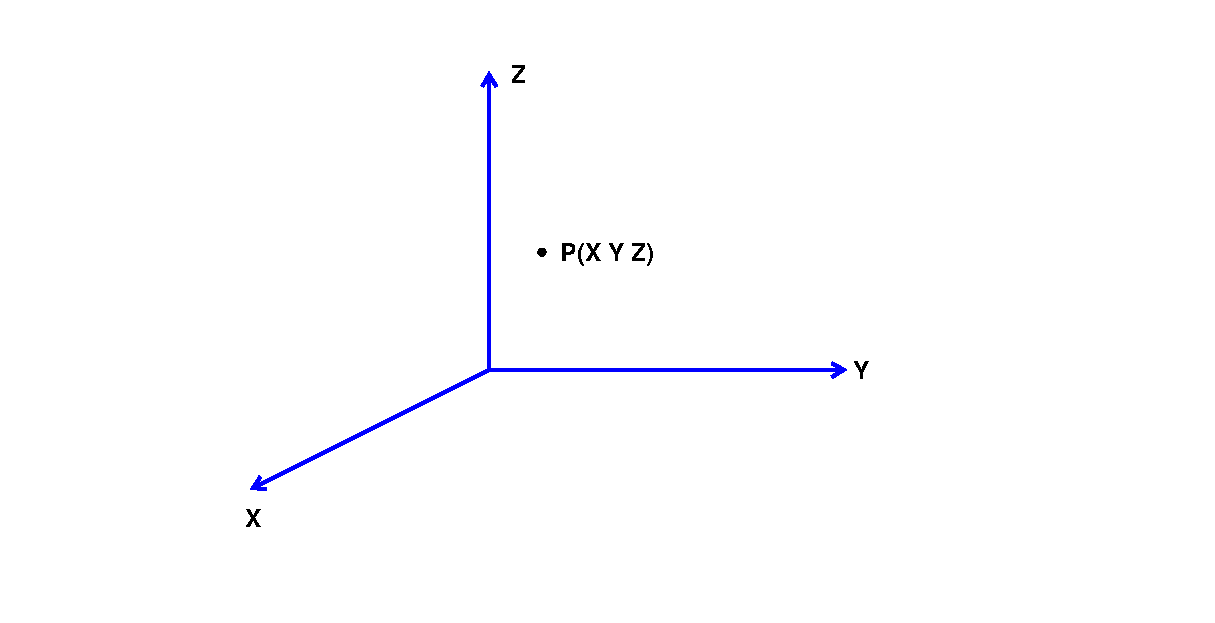
\epsfig{file=eps/base090-1.eps,width=10cm}
      \caption{{\tt GEANT} reference system}
      \label{fg:base090-1}
\end{figure}

Tracking is performed in the {\tt MARS} and the input position for
user routines such as the magnetic field routine is given in this
system.

\section{The local reference systems ({\tt MRS} and {\tt DRS})}
 
As explained in {\tt [GEOM001]}, the setup is
described via the definition of an initial volume inside which all
the others will be positioned. In {\tt GEANT} terminology, each time
a volume has contents, created either via division or by positioning 
other volumes inside, it is called a {\tt MOTHER}. The volumes contained
are called {\tt DAUGHTER}s, and they, in turn, can contain volumes to
a depth of 15 levels. This is sometimes referred to as a {\it Russian doll}
geometry.
 
Every volume defined in {\tt GEANT} has a reference system attached to
it (see {\tt GEOM} section). When this volume has contents, this
is referred to as the {\tt M}other {\tt R}eference {\tt S}ystem
({\tt MRS}, with origin in O$_m$). Daughters
are positioned inside the mother with respect to the {\tt MRS}. The 
{\tt MRS} of the first volume defined, containing all the others, is
nothing else than the {\tt MARS}.

Each one of the daughters has its own reference system, which is referred
to as the {\tt D}aughter {\tt R}eference {\tt S}ystem, or {\tt DRS} with
origin in O$_d$. 

The transformation of a point from the {\tt MRS} (V$_m$)
to the {\tt DRS} (V$_d$), at any level, is performed using a rotation 
matrix $[R]$ and a translation vector $T$ via the relation :
     \[ V_d  =[ R ](V_m -T) \]
The components of $T$ are the projections of the vector  $ (O_m, O_d) $
onto the {\tt MRS} axes.
The rotation matrices are computed from
the spherical angles of each of the axes of the
daughter reference systems ({\tt I, II, III})
with respect to the mother reference system ({\tt 1, 2, 3}).
The spherical angles $\Theta$ and $\Phi$ of a
direction $D$ are defined as follows :
\begin{DLtt}{MMMMM}
\item[$\Theta$]     is the angle formed by the axis 3 and D
                 ($0^{\circ}\;<\;\Theta\;<\;180^{\circ}$).
\item[$\Phi$]      is the angle formed by the axis 1 and the projection
                of D onto the plane defined by the axes 1 and 2
                 ($0^{\circ}\;<\;\Phi\;<\;360^{\circ}$).
\end{DLtt}
Examples are given in {\tt [GEOM200]}.
The various rotation matrices required for a given setup must be
defined by the user during the initialisation stage.
A number is assigned to each matrix {\tt [GEOM200]}.
The translation vector and the number of the rotation
matrix are specified by the user when the volumes are
positioned inside their mother {\tt [GEOM110]}.

\section{Physical units}
 
Unless otherwise specified, the following units are
used throughout the program:
centimeter, second, kilogauss, GeV, GeV c$^{-1}$ (momentum), 
GeV c$^{-2}$ (mass) and degree.

%%%%%%%%%%%%%%%%%%%%%%%%%%%%%%%%%%%%%%%%%%%%%%%%%%%%%%%%%%%%%%%%%%%
%                                                                 %
%  GEANT manual in LaTeX form                                     %
%                                                                 %
%  Michel Goossens (for translation into LaTeX)                   %
%  Version 1.00                                                   %
%  Last Mod. Jan 24 1991  1300   MG + IB                          %
%                                                                 %
%%%%%%%%%%%%%%%%%%%%%%%%%%%%%%%%%%%%%%%%%%%%%%%%%%%%%%%%%%%%%%%%%%%
\Documentation{R.Brun, S.Ravndal}  
\Submitted{01.10.84}    \Revised{10.03.94}
\Version{Geant 3.21}\Routid{BASE100}
\Makehead{Examples of GEANT application}
This section contains a skeleton of a standard user program {\tt GEXAMP}
to use the
{\tt GEANT} system. More detailed examples can be found in the
standard examples {\tt GEXAM1 - 6}. The recommended user routines
are indicated in bold characters and will be explained more in detail
in the following.

\begin{multicols}{2}
\footnotesize
\begin{XMP}
      PROGRAM GEXAMP
      PARAMETER (NGBANK=50000, NHBOOK=5000)
      COMMON/GCBANK/Q(NGBANK)
      COMMON/PAWC  /H(NHBOOK)
C--> {\sl Initialises {\tt HBOOK} and {\tt GEANT} memory}
      CALL GZEBRA( NGBANK)
      CALL HLIMIT(-NHBOOK)
C--> {\sl Open graphics system}
      CALL HPLINT(0)
      CALL IGMETA(8,0)
C--> {\sl {\tt GEANT} initialisation}
      CALL {\bf UGINIT}
C--> {\sl Start events processing}
      CALL GRUN
C--> {\sl End of Run}
      CALL {\bf UGLAST}
      END
*-----------------------------------------------
      SUBROUTINE {\bf UGINIT}
C--> {\sl Initialise {\tt GEANT}}
      CALL GINIT
C--> {\sl Read data records}
      OPEN(4,FILE='gcards.dat',STATUS='UNKNOWN')
      CALL GFFGO
C--> {\sl Initialise data structure}
      CALL GZINIT
C--> {\sl Initialise graphics}
      CALL GDINIT
      IF(NRGET.GT.0) THEN
C--> {\sl Read data structures from file}
         CALL GRFILE(1,'mygeom.dat','I')
      ELSE
C--> {\sl Particle table initialisation}
         CALL GPART
C--> {\sl Geometry and materials description}
         CALL UGEOM
      ENDIF
C--> {\sl Energy loss and cross-sections tables}
      CALL GPHYSI
      IF(NRSAVE .GT. 0) THEN
C--> {\sl Save permanent data structures} 
         CALL GRFILE(2,'mysave.dat','NO')
      ENDIF
C--> {\sl Print banks}
      CALL GPRINT('MATE',0)
      CALL GPRINT('TMED',0)
      CALL GPRINT('VOLU',0)
C--> {\sl Book histograms} 
      END
*-----------------------------------------------
      SUBROUTINE {\bf UGEOM}
C--> {\sl Defines material, tracking media }
C--> {\sl and geometry.}
C--> {\sl Close geometry banks.}
      CALL GGCLOS
      END
*-----------------------------------------------
      SUBROUTINE {\bf GUKINE}
C--> {\sl Generates kinematics}
C--> {\sl Data card {\tt KINE} itype x y z px py pz}
+SEQ, GCFLAG.
+SEQ, GCKINE.
      CALL GSVERT(PKINE,0,0,0,0,NVERT)
      CALL GSKINE(PKINE(4),IKINE,NVERT,0,0,NT)
C--> {\sl Print kinematic}
      IF (IDEBUG.NE.0) THEN
         CALL GPRINT('VERT',0)
         CALL GPRINT('KINE',0)
      END IF
      END
*-----------------------------------------------
      SUBROUTINE {\bf GUSTEP}
C--> {\sl Called at the end of each tracking }
C--> {\sl step.}
+SEQ, GCKINE.
C--> {\sl Debug event}
      CALL GDEBUG
C--> {\sl Store the created particles} 
      IF (NGKINE.GT.0) CALL GSKING (0)
      END
*-----------------------------------------------
      SUBROUTINE {\bf UGLAST}
C--> {\sl Termination routine} 
C--> {\sl Print histograms and statistics}
      CALL GLAST
C--> {\sl Close {\tt HIGZ/GKS} file}
      CALL IGEND
      END
\end{XMP}
\end{multicols}

\section{Notes}
\begin{itemize}
\item Whenever possible {\tt GEANT} makes use of the {\tt ZEBRA} store
for large data structures. This allows it to adapt the size of the program
data portion
to the size of the problem. The total amount of space required depends
on the application. {\tt GEANT} can run with as little as 50,000 words
or less, but for large detectors it is not uncommon to 
declare stores of several million words. The call to \Rind{GZEBRA}
initialises the common \FCind{/GCBANK/} to receive the {\tt GEANT}
data structures. This call is necessary before any other routine of
the {\tt GEANT} system is called.
\item The call to \Rind{HLIMIT} initialises the {\tt ZEBRA} system
to use the \FCind{/PAWC/} common block for the {\tt HBOOK} histogram
package. The size of the common depends on the number and size of the
plot requested. The {\tt ZEBRA} system must be initialised only once,
and the negative argument to \Rind{HLIMIT} prevents a second
initialisation of the system.
The \Rind{HLIMIT} call has to be placed {\bf after} the call
to \Rind{GZEBRA} and the argument has to be the dimension of the 
\FCind{/PAWC/} common block with a negative sign in front. 
\item
The main program is intended for {\it batch} applications,
while to run the simulation interactively, the interactive main program
called \Rind{GXINT} should be linked in front of the user code.
\item The program shown will require the graphic libraries in the
link sequence. Often, for batch production or for
small tests, graphics is not needed, and not loading the graphics
code makes the program smaller. To avoid loading graphic routines
the calls to \Rind{IGINIT}, \Rind{IGMETA}, \Rind{IGEND}, \Rind{GDINIT}
and \Rind{GDEBUG} should be removed. 

If, on the other hand, the user is interested in including the routine
\Rind{GDEBUG} and in excluding graphics at the same time, then the
following routine should be included in the code:
\begin{verbatim}
      SUBROUTINE GDCXYZ
      ENTRY IGSA
      ENTRY GDTRAK
      END
\end{verbatim}

which will avoid every reference to the graphics routines from \Rind{GDEBUG}.

\item The user code to define the {\it tracking media} and the geometry
of the setup should be inside the routine \Rind{UGEOM}. The pre-initialised
data structured can be read from disk, but it is recommended to call 
\Rind{GPHYSI} in any case, to initialise the cross-section tables. An 
example of a full material, geometry and detector design is given below
and has been extracted from the example {\tt GEXAM3}. Here only major
calls are shown, the redundant parts can be found in the source code
of \Rind{UGEOM} in {\tt GEXAM3}. 

The example shows the basic concept in 
{\tt GEANT}. First material parameters are defining the properities of
a detector material calling the subroutine \Rind{GSMATE}. 
Here in addition to the 16 predefined materials, the material definition of
Calcium is examplary shown. More information towards the predefined materials
and further use of material definition routines can be found in the 
section {\tt CONS001 - CONS101}.
Then tracking parameters are associated to the materials, defining
a so called tracking medium. Each {\tt GEANT}  volume must be 
associated to an existing tracking medium. Here in the example the
tracking medium {\tt 'TARGET'} is defined to exist of Calcium.
 
In the example shown below several
detector volumes are defined using the subroutine \Rind{GSVOLU}.
The defined volume have associated parameters of name, shape,
tracking medium and shape parameters.
In this example the volume {\tt 'TGT '} consists of the 
previously defined tracking medium {\tt 'TARGET'}.The 
volumes (and if necessary identical copies of them)
are then positioned according to the detector geometry. The 
volumes are positioned on the same level, or inside each other. By
setting the parameter {\tt ONLY} or  {\tt MANY} in the call of \Rind{GSPOS} 
the user has the opportunity to tell either {\tt GEANT} the logical
volume structure and to apply boolean operations (cutting, joining and
intersection) between two positioned volumes. More information about
the concept in defining volumes and positioning can be retrieved from
the section {\tt GEOM}. 

Finally the user is required to classify into sets all
sensitive detectors (defined as those volume defined as
detector via \Rind{GSDET} and other related routines, for which 
he wants to store hits in the hit data structure {\tt JHITS}.
\begin{multicols}{2}
\footnotesize
\begin{XMP}
      SUBROUTINE {\bf UGEOM}
+SEQ,GCLIST
+SEQ,GCONSP
      COMMON/DLSFLD/ISWFLD,FLDVAL
C--> {\sl Defining material parameters}
C--> {\sl Defining geometry parameters}
C--> {\sl Defining positioning parameters}
C--> {\sl Data statements, left out here, to}
C--> {\sl Define materials and mixtures}
      CALL GSMATE(17,'CALCIUM$',
     + 40.08,20.,1.55,10.4,23.2,0,0)
C--> {\sl .......}
C--> {\sl further material an mixture definitions}
C--> {\sl .......}
C--> {\sl Defining tracking media}
      CALL GSTMED( 2,'TARGET    $',
     + 17,0,0,0.,10.,.2,.1,.001,.5,0,0)
C--> {\sl .......}
C--> {\sl defining further media}
C--> {\sl .......}
C--> {\sl Define the reference frame}
      CALL GSVOLU
     +     ('CAVE','BOX ',1,CAVPAR,3,ICAVE)
C--> {\sl The targe box is shifted by 100 cm}
C--> {\sl in the cave.}
      CALL GSVOLU
     +     ('TGT ','BOX ',2,TGTPAR,3,ITGT )
      CALL GSVOLU
     +     ('TBIN','TRD1',3,TBIPAR,4,ITBIN)
      CALL GSVOLU
     +     ('TBOU','TRD1',4,TBOPAR,4,ITBOU)
      CALL GSVOLU
     +     ('ARM ','TRD1',1,ARMPAR,4,IARM)
      CALL GSVOLU
     +     ('FDIN','BOX ',9,FDIPAR,3,IFDIN)
      CALL GSVOLU
     +     ('FDOU','BOX ',4,FDOPAR,3,IFDOU)
C--> {\sl Define drift wire planes}
      CALL GSVOLU
     +     ('FSP ','BOX ',13,FDIPAR,3,IFSP)
C--> {\sl .......}
C--> {\sl further geometry definitions}
C--> {\sl .......}
C--> {\sl Positioning the daughter volumes in}
C--> {\sl their mother volume.}
      CALL GSPOS
     + ('TGT ',1,'TBIN', 0., 0.,-5.08,0,'ONLY')
      CALL GSPOS
     + ('TGT ',2,'TBIN', 0., 0.,-2.54,0,'ONLY')
      CALL GSPOS
     + ('TGT ',3,'TBIN', 0., 0., 0.  ,0,'ONLY')
      CALL GSPOS
     + ('TGT ',4,'TBIN', 0., 0., 2.54,0,'ONLY')
      CALL GSPOS
     + ('TGT ',5,'TBIN', 0., 0., 5.08,0,'ONLY')
      CALL GSPOS
     + ('TBIN',1,'TBOU', 0., 0.,   0.,0,'ONLY')
      CALL GSPOS
     + ('TBOU',1,'CAVE', 0., 0.,  ZTG,0,'ONLY')
      CALL GSPOS
     + ('ARM ',1,'CAVE',XLARM,0.,ZLARM,1,'ONLY')
      CALL GSPOS
     + ('ARM ',2,'CAVE',XRARM,0.,ZRARM,2,'ONLY')
      CALL GSPOS
     + ('FDOU',1,'ARM ',0.,0., DFDO  ,0,'ONLY')
      CALL GSPOS
     + ('FDIN',1,'FDOU',0.,0., 0.    ,0,'ONLY')
      CALL GSPOS
     + ('FSP ',1,'FDIN',0.,0.,-2.9975,0,'ONLY')
C--> {\sl .......}
C--> {\sl positioning of further volumes}
C--> {\sl .......}
C--> {\sl Print the stored definitions}
      CALL GLOOK('VOLU',LPRIN,NPRIN,ILOOK)
      IF(ILOOK.NE.0) CALL GPVOLU(0)
      CALL GLOOK('ROTM',LPRIN,NPRIN,ILOOK)
      IF(ILOOK.NE.0) CALL GPROTM(0)
      CALL GLOOK('TMED',LPRIN,NPRIN,ILOOK)
      IF(ILOOK.NE.0) CALL GPTMED(0)
      CALL GLOOK('MATE',LPRIN,NPRIN,ILOOK)
      IF(ILOOK.NE.0) CALL GPMATE(0)
      CALL GLOOK('PART',LPRIN,NPRIN,ILOOK)
      IF(ILOOK.NE.0) CALL GPPART(0)
C--> {\sl Clean up volume banks and perform}
C--> {\sl optimization}
      CALL GGCLOS
C--> {\sl Define sensitive detector parts}
      CALL GSDET
     &('DRFT','FSP ',2,NAFD ,NBITSV,1,100,
     &100,IDRFT,IFD )
C--> {\sl Define hit parameters}
      CALL GSDETH('DRFT','FSP ',9,NAMESH,
     &NBITSH,ORIG,FACT)
      RETURN
      END
\end{XMP}
\end{multicols}





\item It is convenient to store the input data records (see {\tt [BASE040]})
in an auxiliary file ({\tt gcards.dat} in the example). This allows to
have a standard input file and to overwrite selected input data records
as needed.
If, for instance, the standard {\tt gcards.dat} file contains the record
{\tt TRIG 1000} and a short test run is requested this can be obtained
with the following input:
\begin{verbatim}
READ 4
TRIG 10
STOP
\end{verbatim}
the first line instructs {\tt FFREAD} to open and process the file
connected with logical unit 4, and the second line (re-)defines the
number of events to be processed. The {\tt STOP} command ends the 
{\tt FFREAD} processing of the input.
\item 
In the above
example the common blocks have not been expanded in the code. The notation
used is the one of the {\tt PATCHY}/{\tt CMZ}~\cite{bib-PATCHY,bib-CMZ}
code management systems. These products, among other things, can
run as pre-processors, replacing the {\tt +SEQ,...}
instructions with the corresponding code fragments. Users are strongly
recommended to use these systems to include {\tt GEANT} common blocks
in their code. 

Long experience in supporting {\tt GEANT} users has shown that, as the
user program grows, typing errors in the insertion of the common blocks
{\it by hand} become very common, but difficult to find. The investment
needed to learn a code management system at the user level is usually 
negligible compared with the time and energy needed in hunting a
problem introduced by a mistyped common.
\end{itemize}

%%%%%%%%%%%%%%%%%%%%%%%%%%%%%%%%%%%%%%%%%%%%%%%%%%%%%%%%%%%%%%%%%%%
%                                                                 %
%  GEANT manual in LaTeX form                                     %
%                                                                 %
%  Version 1.00                                                   %
%  Last Mod.  8 June 1993 1300   MG                               %
%                                                                 %
%%%%%%%%%%%%%%%%%%%%%%%%%%%%%%%%%%%%%%%%%%%%%%%%%%%%%%%%%%%%%%%%%%%
\Origin {R.Brun} 
\Submitted{01.06.83}  \Revised{16.12.93}
\Version{Geant 3.16}\Routid{BASE110}
\Makehead{The system initialisation routines}
 
\Shubr{GZEBRA}{(NZ)}
 
Initialises the {\tt ZEBRA} memory manager to use the common \FCind{/GCBANK/}
to store the {\tt GEANT} data structures.
\begin{DLtt}{MMMMMMMM}
\item[NZ] ({\tt INTEGER}) size of the \FCind{/GCBANK/} common as it is
dimensioned in the main program.
\end{DLtt}
The size of the dynamic memory is set to {\tt NZ-30}. The common
\FCind{/GCBANK/} must be dimensioned in the main program.
{\tt ZEBRA}~\cite{bib-ZEBRA} must be initialised only once. The call to the
{\tt HBOOK} initialisation routine \Rind{HLIMIT} tries to initialise
{\tt ZEBRA} as well, and this will cause a program abort. To avoid this,
\Rind{HLIMIT} must be called {\bf after} \Rind{GZEBRA} and its argument
must be a negative number whose absolute value is the size of the
\FCind{/PAWC/} common containing the histograms. This is shown in the
example of main program given in {\tt[BASE100]}.

\Shubr{GINIT}{}
Presets labelled common block variables to default values.
See {\tt[BASE030]} for more information.

\Shubr{GFFGO}{}
Reads a set of data records via the {\tt FFREAD} package.
See {\tt[BASE040]} for more information on the possible data records.
\Rind{GFFGO} must be called after \Rind{GINIT}.

\Shubr{GZINIT}{}

Initialises the {\tt ZEBRA} permanent data structures in division
2 of the {\tt GEANT} main store in common  \FCind{/GCBANK/}.
Creates the user long term division (index {\tt IXCONS})
(minimum size {\tt 2000}, maximum size {\tt 8*NZEBRA/10}).
The {\tt ZEBRA} division {\tt IXDIV} is reserved for the event data structures
and the division {\tt IXCONS} for the initialisation data structures.
Allocates 5200 words of working space.
Initialises the link areas and a default run header bank {\tt JRUNG
[BASE299]}. Defines banks format for I/O.
\Rind{GZINIT} must be called after \Rind{GFFGO}.
 
A layout of the dynamic store is shown in fig \ref{fg:base110-1}.

\begin{figure}[hbt]
      \centering
      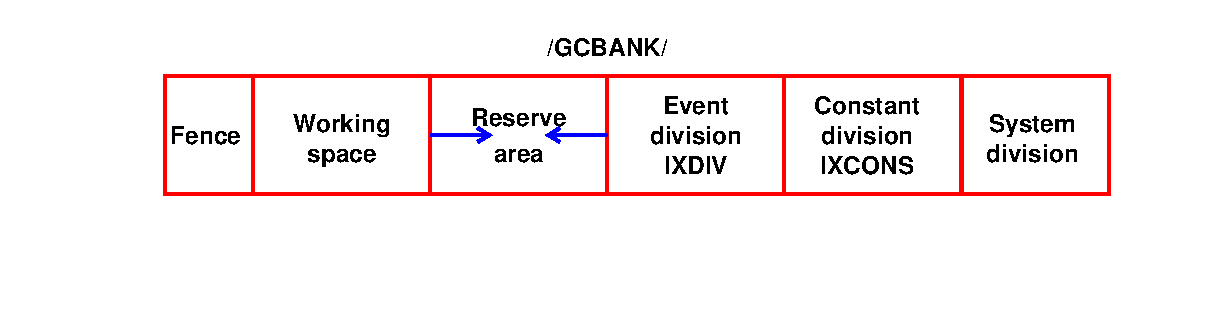
\epsfig{file=eps/base110-1.eps,width=16cm}
      \caption{Layout of the dynamic store}
      \label{fg:base110-1}
\end{figure}

\Shubr{GDINIT}{}
This routine
initialises the {\tt GEANT} drawing package {\tt[DRAW001]} and it has
to be called before any other graphic routine. {\tt GEANT} uses the
CERN-developed {\tt HIGZ}~\cite{bib-HIGZ} graphic library, and this
has to be initialised before the call to \Rind{GDINIT}.
In the example given
in {\tt [BASE100]} the routines \Rind{IGINIT} and \Rind{IGMETA}
are used. Alternatively, the routine \Rind{HPLINT} from HPLOT~\cite{bib-HPLOT}
can be used. This routine calls the appropriate procedures from {\tt HIGZ} to 
initialise the underlaying graphics system. At the moment {\tt HIGZ} can 
use several flavours of GKS~\cite{bib-gks2d,bib-gks3d,bib-GKS1}
and {\tt X11} and it is available on all machines where the CERN Program
Library has been installed.

\Shubr{GPHYSI}{}
Completes the data structure {\tt JMATE}, (see {\tt [PHYS100]}) calculating the
cross-section and stopping power tables.

\Shubr{GBHSTA}{}
Initialises the standard histograms requested by the user via the
data record {\tt HSTA}.
The following histogram keywords may be used :
\begin{DLtt}{MMMMMMMM}
\item[TIME]    time per event;
\item[SIZE]     size of division {\tt IXDIV} per event;
\item[MULT]    total number of tracks per event;
\item[NTRA]    number of {\it long life} tracks per event;
\item[STAK]    maximum stack size per event.
\end{DLtt}

\Rind{GBHSTA} should be called after \Rind{GFFGO}.

\Shubr{GGCLOS}{}
This routine has to be called at the end of the definition
of the geometry by the user, after thal all volumes have been defined
and positioned and all detectors defined. 
Failure to call this routine will prevent
the {\tt GEANT} system from working correctly. Main tasks of this routine
are:
\begin{itemize}
\item close the geometry package;
\item complete the {\tt JVOLUM} data structure;
\item process the detector definition provided by the user;
\item prepare the tables for the tracking speed optimisation requested
by the user via the \Rind{GSORD} routine or the {\tt OPTI} data record.
\end{itemize}

%%%%%%%%%%%%%%%%%%%%%%%%%%%%%%%%%%%%%%%%%%%%%%%%%%%%%%%%%%%%%%%%%%%
%                                                                 %
%  GEANT manual in LaTeX form                                     %
%                                                                 %
%  Version 1.00                                                   %
%  Last Mod.  8 June 1993 1300   MG                               %
%                                                                 %
%%%%%%%%%%%%%%%%%%%%%%%%%%%%%%%%%%%%%%%%%%%%%%%%%%%%%%%%%%%%%%%%%%%
\Origin{R.Brun}     
\Submitted{01.06.83}   \Revised{26.10.93}
\Version{Geant 3.16}\Routid{BASE200}
\Makehead{Steering routines for event processing}
\Shubr{GRUN}{}
Main routine to control a run of events. The following flow chart is only 
valid for the {\it batch} execution mode. For interactive applications, 
see section {\tt XINT}. A schematic description of the routine is shown 
in fig.~\ref{fg:base200-1}.
 
\begin{figure}[hbt]
      \centering
      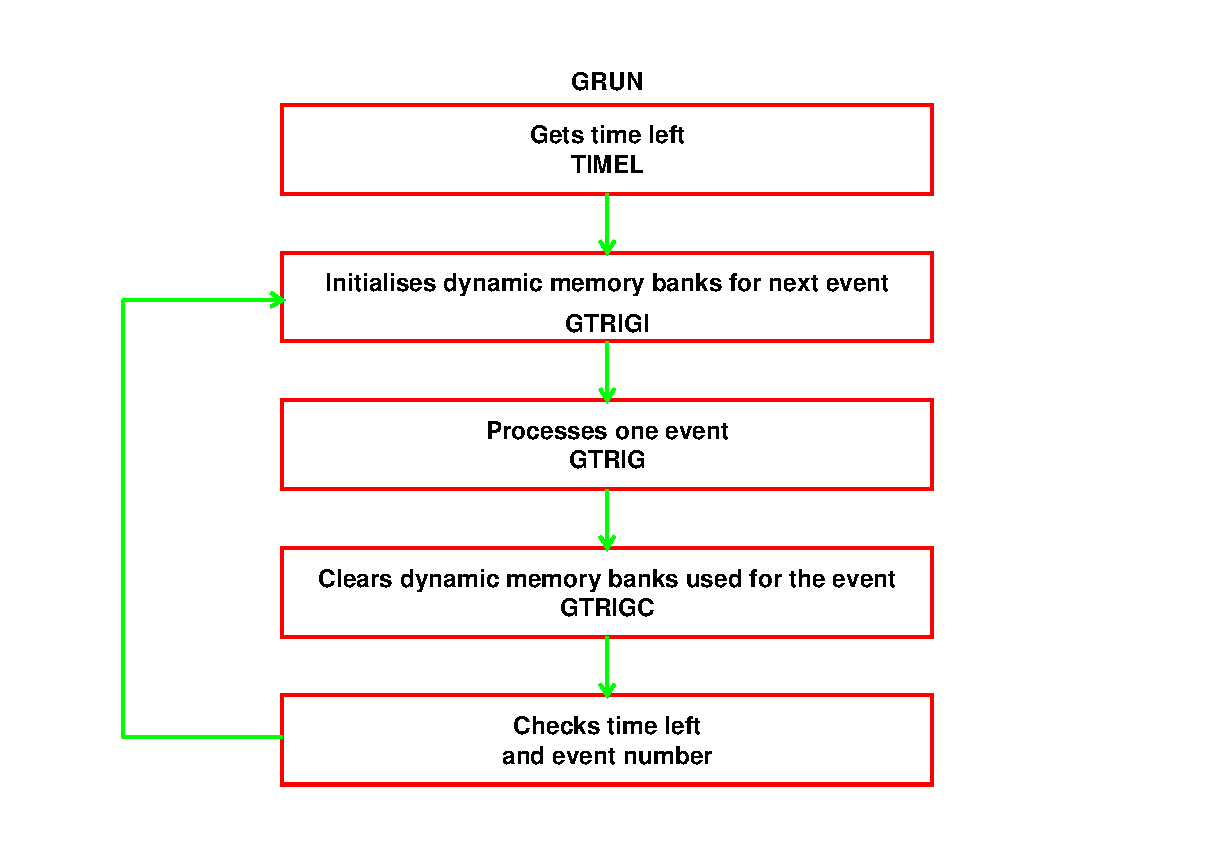
\epsfig{file=eps/base200-1.eps,width=16cm}
      \caption{Flow of the {\tt GRUN} routine.}
      \label{fg:base200-1}
\end{figure}

\Shubr{GTRIGI}{}
Initialisation routine for event processing:
\begin{itemize}
\item resets to 0 the flag {\tt IEOTRI} in \FCind{/GCFLAG/} and the counters
{\tt NTRACK} and {\tt NVERTX} in \FCind{/GCNUM/};
\item sets the debug flag
{\tt IDEBUG} in \FCind{/GCFLAG/}
to the value required for the current event;
\item creates a default header bank
{\tt JHEAD} for current event {\tt [BASE299]};
\item prints the sequence number, the event number and the random number
generator seeds,
under control of the flag {\tt ITEST} (data record {\tt DEBU}).
\end{itemize}
 
\Shubr{GTRIG}{}
 
Steering routine to process one event (trigger).
A schematic description of the routine is shown 
in fig.~\ref{fg:base200-2}.
 
\begin{figure}[hbt]
      \centering
      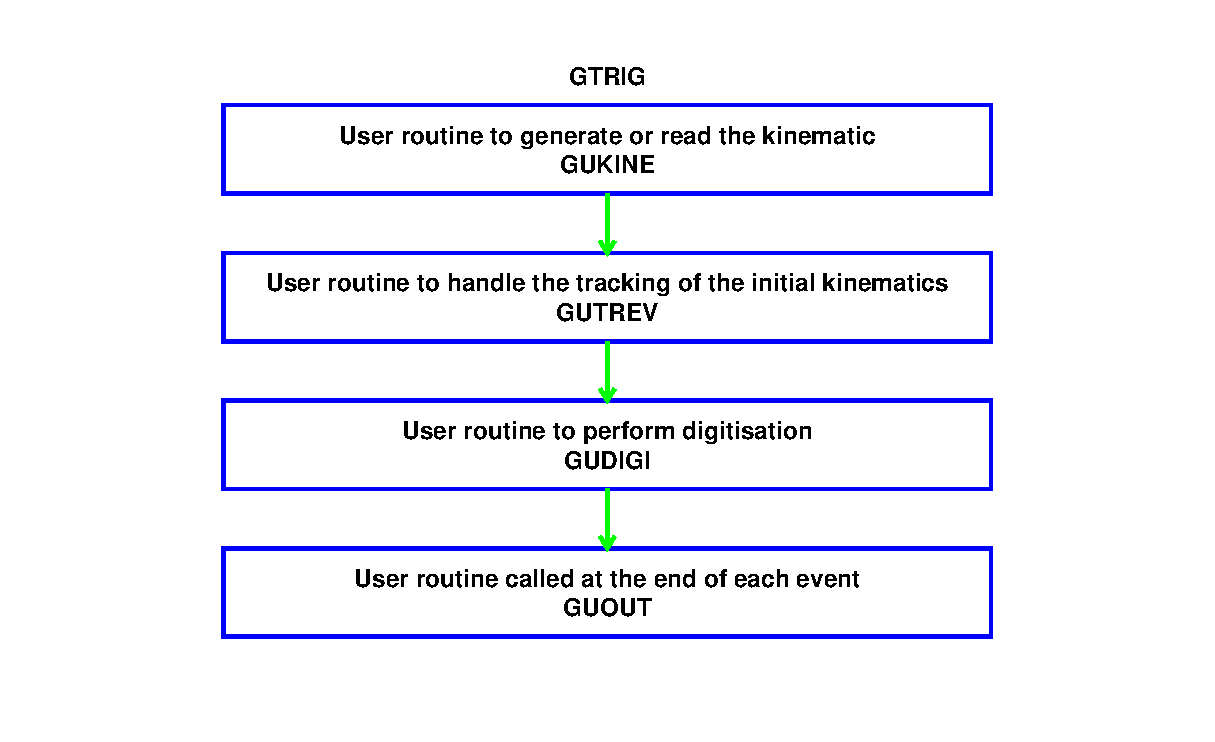
\epsfig{file=eps/base200-2.eps,width=16cm}
      \caption{Flow of the {\tt GRUN} routine.}
      \label{fg:base200-2}
\end{figure}

Default routines provided by {\tt GEANT} are dummy.

\Shubr{GTRIGC}{}
The event division {\tt IXDIV} is cleared. The space
used by the current event may be used by the next one.
 

%%%%%%%%%%%%%%%%%%%%%%%%%%%%%%%%%%%%%%%%%%%%%%%%%%%%%%%%%%%%%%%%%%%
%                                                                 %
%  GEANT manual in LaTeX form                                     %
%                                                                 %
%  Michel Goossens (for translation into LaTeX)                   %
%  Version 1.00                                                   %
%  Last Mod. Jan 24 1991  1300   MG + IB                          %
%                                                                 %
%%%%%%%%%%%%%%%%%%%%%%%%%%%%%%%%%%%%%%%%%%%%%%%%%%%%%%%%%%%%%%%%%%%
\Origin{M.Maire}
\Submitted{14.12.93}  \Revised{14.12.93}
\Version{Geant 3.16}\Routid{BASE280}

\Makehead{Storing and retrieving JRUNG and JHEAD information}

\Shubr{GSRUNG}{(NUBUF,UBUF,IADR*)}
\begin{DLtt}{MMMMMMMM}
\item[NUBUF] ({\tt INTEGER}) number of user words;
\item[UBUF] ({\tt REAL}) array of user words;
\item[IADR] ({\tt INTEGER}) position where information is stored in the
user bank of the {\tt JRUNG} structure.
\end{DLtt}

This routine stores the first {\tt NUBUF} words of array {\tt BUF} in the
user bank attached to the structure {\tt JRUNG} (see {\tt [BASE299]}),
starting at location {\tt IADR+1}.
On exit {\tt IADR} is set to {\tt IADR+NUBUF}, allowing subsequent filling. 
This allows effectively 
to {\it add} information to the current {\tt JRUNG} bank, whether or not it has 
already an user buffer.

\Shubr{GFRUNG}{(NWRUNG*,IRUNG*,NUBUF*,UBUF*)}
\begin{DLtt}{MMMMMMMM}
\item[NWRUNG] ({\tt INTEGER}) number of words in {\tt JRUNG} bank;
\item[IRUNG] ({\tt REAL}) content of {\tt JRUNG} bank;
\item[NUBUF] ({\tt INTEGER}) number of user words;
\item[UBUF] ({\tt REAL}) array of user words;
\end{DLtt}

This routine retrieves the content of the {\tt JRUNG} bank and of the
user information added, if any.

\Shubr{GPRUNG}{}

This routine prints the content of the {\tt JRUNG} bank and of the
user information added, if any.

\Shubr{GSHEAD}{(NUBUF,UBUF,IADR*)}
\begin{DLtt}{MMMMMMMM}
\item[NUBUF] ({\tt INTEGER}) number of user words;
\item[UBUF] ({\tt REAL}) array of user words;
\item[IADR] ({\tt INTEGER}) position where information is stored in the
user bank of the {\tt JHEAD} structure.
\end{DLtt}

This routine stores the first {\tt NUBUF} words of array {\tt BUF} in the
user bank attached to the structure {\tt JHEAD} (see {\tt [BASE299]}),
starting at location {\tt IADR+1}.
On exit {\tt IADR} is set to {\tt IADR+NUBUF}, allowing subsequent filling. 
This allows effectively 
to {\it add} information to the current {\tt JHEAD} bank, whether or not it has 
already an user buffer.

\Shubr{GFHEAD}{(NWHEAD*,IHEAD*,NUBUF*,UBUF*)}
\begin{DLtt}{MMMMMMMM}
\item[NWHEAD] ({\tt INTEGER}) number of words in {\tt JHEAD} bank;
\item[IHEAD] ({\tt REAL}) content of {\tt JHEAD} bank;
\item[NUBUF] ({\tt INTEGER}) number of user words;
\item[UBUF] ({\tt REAL}) array of user words;
\end{DLtt}

This routine retrieves the content of the {\tt JHEAD} bank and of the
user information added, if any.

\Shubr{GPHEAD}{}

This routine prints the content of the {\tt JHEAD} bank and of the
user information added, if any.

%%%%%%%%%%%%%%%%%%%%%%%%%%%%%%%%%%%%%%%%%%%%%%%%%%%%%%%%%%%%%%%%%%%
%                                                                 %
%  GEANT manual in LaTeX form                                     %
%                                                                 %
%  Michel Goossens (for translation into LaTeX)                   %
%  Version 1.00                                                   %
%  Last Mod. Jan 24 1991  1300   MG + IB                          %
%                                                                 %
%%%%%%%%%%%%%%%%%%%%%%%%%%%%%%%%%%%%%%%%%%%%%%%%%%%%%%%%%%%%%%%%%%%
\Origin{R.Brun, F.Bruyant}  
\Submitted{01.10.84}  \Revised{14.12.93}
\Version{Geant 3.16}\Routid{BASE299}
\Makehead{The banks JRUNG and JHEAD}
Run bank {\tt JRUNG}:  1 user link, 30 data words
 
\vspace{0.7cm}
\begin{tabular}{r@{}ll}
\hspace{2cm} {\tt LQ(JRUNG} &{\tt-1)} &user link      \\
                                                      \\
{\tt IQ(JRUNG}&{\tt+1)} &{\tt IDRUN} (Run number)           \\
&{\tt+2 \dots +10)} &Reserved for user applications    \\
&{\tt+11)} &creation date for {\tt INIT} data structures \\
&{\tt+12)} &creation time for {\tt INIT} data structures \\
&{\tt+13)} &creation date for {\tt KINE}                 \\
&{\tt+14)} &creation time for {\tt KINE}                 \\
&{\tt+15)} &creation date for {\tt HITS}                 \\
&{\tt+16)} &creation time for {\tt HITS}                 \\
&{\tt+17)} &creation date for {\tt DIGI}                 \\
&{\tt+18)} &creation time for {\tt DIGI}                 \\
&{\tt+19)} &\parbox[t]{10cm}{{\tt NRNDM(1)}
First seed for the random number generator 
at the end of the last event generated}\\
&{\tt+20)} &\parbox[t]{10cm}{{\tt NRNDM(2)}
Second seed for the random number generator 
at the end of the last event generated}\\
&{\tt+21)} &{\tt GEANT} version number when {\tt INIT} created  \\
&{\tt+22)} &{\tt ZEBRA} version number when {\tt INIT} created  \\
&{\tt+23)} &{\tt GEANT} version number when {\tt KINE} created  \\
&{\tt+24)} &{\tt ZEBRA} version number when {\tt KINE} created  \\
&{\tt+25)} &{\tt GEANT} version number when {\tt HITS} created  \\
&{\tt+26)} &{\tt ZEBRA} version number when {\tt HITS} created  \\
&{\tt+27)} &{\tt GEANT} version number when {\tt DIGI} created  \\
&{\tt+28)} &{\tt ZEBRA} version number when {\tt DIGI} created  \\
&{\tt+29)} &\parbox[t]{10cm}{{\tt IEVENT} event sequence number 
at the end of the last generated event} \\
\end{tabular}
\vspace{0.7cm}
 
Header bank {\tt JHEAD}: 1 user link, {\tt NHEAD(=10)} data words
\vspace{0.7cm}
 
\begin{tabular}{r@{}lll}
\hspace{2cm} {\tt LQ(JHEAD} &{\tt-1)} &user link      \\
                                                       \\
{\tt IQ(JHEAD}&{\tt+1)} &{\tt IDRUN} &Run number         \\
&{\tt+2)} &{\tt IDEVT} &Event number                  \\
&{\tt+3)} &{\tt NRNDM(1)} &\parbox[t]{8.1cm}{Value of random number generator 
first seed at the beginning of the event} \\
&{\tt+4)} &{\tt NRNDM(2)} &\parbox[t]{8.1cm}{Value of random number generator 
second seed at the beginning of the event} \\
&{\tt+5 \dots 10)} & & Reserved for user applications         \\
\end{tabular}

%%%%%%%%%%%%%%%%%%%%%%%%%%%%%%%%%%%%%%%%%%%%%%%%%%%%%%%%%%%%%%%%%%%
%                                                                 %
%  GEANT manual in LaTeX form                                     %
%                                                                 %
%  Version 1.00                                                   %
%  Last Mod.  8 June 1993 1300   MG                               %
%                                                                 %
%%%%%%%%%%%%%%%%%%%%%%%%%%%%%%%%%%%%%%%%%%%%%%%%%%%%%%%%%%%%%%%%%%%
\Documentation{R.Brun}  
\Submitted{01.10.84} \Revised{08.11.93}
\Version{Geant 3.16}\Routid{BASE300}
\Makehead{Example of user termination routine}
\begin{verbatim}
    SUBROUTINE UGLAST
*
+SEQ,GCLIST
*
*       Call standard GEANT termination routine
    CALL GLAST
*
*       Terminate graphics
    CALL HPLEND
*
*       Close I/O buffers
    IF(NGET .NE. 0 .OR. NSAVE .NE. 0) CALL GCLOSE(0,IER)
*
*       Print histograms
    CALL HISTDO
*
    END
\end{verbatim}
\Shubr{GLAST}{}
Standard {\tt GEANT} termination routine:
\begin{itemize}
\item computes and prints the processing time per event;
\item calls \Rind{MZEND} to print the statistics relative to the current run;
\item if the structure {\tt JGSTAT} has been initialised, calls \Rind{GPSTAT}
{\tt [GEOM700]}.
\end{itemize}

%%%%%%%%%%%%%%%%%%%%%%%%%%%%%%%%%%%%%%%%%%%%%%%%%%%%%%%%%%%%%%%%%%%
%                                                                 %
%  GEANT manual in LaTeX form                                     %
%                                                                 %
%  Version 1.00                                                   %
%  Last Mod.  8 June 1993 1300   MG                               %
%                                                                 %
%%%%%%%%%%%%%%%%%%%%%%%%%%%%%%%%%%%%%%%%%%%%%%%%%%%%%%%%%%%%%%%%%%%
\Origin{R.Brun, F.Carena}
\Submitted{01.10.84}  \Revised{16.12.93}
\Version{Geant 3.16}\Routid{BASE400}
\Makehead{Debugging facilities}
The flags {\tt IDEBUG, ITEST} and {\tt ISWIT(1-10)} are available to
in the
common \FCind{/GCFLAG/} for debug control {\tt [BASE030]}.
The array {\tt ISWIT} is filled through the data record
{\tt SWIT}.
Some flags are used by \Rind{GHEISHA} {\tt [PHYS510]} and
by the routine \Rind{GDEBUG}.

The flag {\tt IDEBUG} is set to 1 in \Rind{GTRIGI} for the events
with sequence number from {\tt IDEMIN} to {\tt IDEMAX}, as specified by
the user on the data record {\tt DEBU}.
If {\tt IDEMIN} is negative, debug is
activated also in the initialisation phase.

The flag {\tt ITEST}, set by the user via the data
record {\tt DEBU}, is also used by \Rind{GTRIGI}.
The sequence number, the event number and the random numbers seeds are
printed at the beginning of each event every {\tt ITEST} from
{\tt IDEMIN} to {\tt IDEMAX}.

\section{Debug of data structures}
The contents of the data structures can be dumped by the routine
\Shubr{GPRINT}{(CHNAME,NUMB)}
\begin{DLtt}{MMMMMMMM}
\item[CHNAME] ({\tt CHARACTER*4}) name of a top level data structure;
\item[NUMB] ({\tt INTEGER}) number of the substructure to be printed, 0 for all.
\end{DLtt}

Examples
\begin{itemize}
\item{\tt CALL GPRINT('KINE',0)} prints all banks {\tt JKINE};
\item{\tt CALL GPRINT('KINE',8)} prints {\tt JKINE} bank for track 8;
\item{\tt CALL GPRINT('VOLU',0)} prints all existing volumes.
\end{itemize}
The following names are recognised:
\begin{center}\tt
DIGI,HITS,KINE,MATE,VOLU,ROTM,SETS,TMED,PART,VERT,JXYZ
\end{center}
\Rind{GPRINT} calls selectively the routines:

\begin{center}
\begin{tabular}{llll}
\Rind{GPDIGI}{\tt ('*','*')} &
\Rind{GPHITS}{\tt ('*','*')} &
\Rind{GPKINE}{\tt (NUMB)}    & 
\Rind{GPMATE}{\tt (NUMB)}    \\
\Rind{GPVOLU}{\tt (NUMB)}    &
\Rind{GPROTM}{\tt (NUMB)}    &
\Rind{GPSETS}{\tt ('*','*')} &
\Rind{GPTMED}{\tt (NUMB)}    \\
\Rind{GPPART}{\tt (NUMB)}    &
\Rind{GPVERT}{\tt (NUMB)}    &
\Rind{GPJXYZ}{\tt (NUMB)}    &
\end{tabular}
\end{center}

These routines can be called directly by the user. In case of {\tt SETS},
{\tt HITS} and {\tt DIGI} the content of all detectors of all sets will
be printed, so {\tt NUMB} is irrelevant.

\section{Debug of events}
The development of an event can be followed via the routine:
\Shubr{GDEBUG}{}

which operates under the control of the {\tt ISWIT} array. It is the
user responsibility to call this routine from \Rind{GUSTEP}. If the
{\tt DEBUG} flag is active, the routine will perform as follows:
\begin{DLtt}{MMMMM}
\item[ISWIT(1)] ~

\begin{DLtt}{MMM}
\item[2]the content of the temporary stack for secondaries in the
common \FCind{/GCKING/} is printed;
\end{DLtt}
\item[ISWIT(2)] ~

\begin{DLtt}{MMM}
\item[1]the current point of the track is stored in the {\tt JDXYZ}
bank via the routine \Rind{GSXYZ};
\item[2]the current information on the track is printed via the
routine \Rind{GPCXYZ};
\item[3]the current step is drawn via the routine
\Rind{GDCXYZ};
\item[4]the current point of the track is stored in the {\tt JDXYZ}
bank via the routine \Rind{GSXYZ}. When the particle stops the track
is drawn via the routine \Rind{GDTRAK}
and the space occupied by the track in the structure {\tt JDXYZ}
released;
\end{DLtt}
\item[ISWIT(3)] ~

\begin{DLtt}{MMM}
\item[1]the current point of the track is stored in the {\tt JDXYZ}
bank via the routine \Rind{GSXYZ}.
\end{DLtt}
\end{DLtt}

%%%%%%%%%%%%%%%%%%%%%%%%%%%%%%%%%%%%%%%%%%%%%%%%%%%%%%%%%%%%%%%%%%%
%                                                                 %
%  GEANT manual in LaTeX form                                     %
%                                                                 %
%  Michel Goossens (for translation into LaTeX)                   %
%  Version 1.00                                                   %
%  Last Mod. Jan 24 1991  1300   MG + IB                          %
%                                                                 %
%%%%%%%%%%%%%%%%%%%%%%%%%%%%%%%%%%%%%%%%%%%%%%%%%%%%%%%%%%%%%%%%%%%
\Origin{R.Brun}
\Submitted{08.08.87}  \Revised{08.11.93}
\Version{Geant 3.16}\Routid{BASE410}
\Makehead{Utility Routines}
 
\Shubr{GLOOK}{(CHNAME,IVECT,N,ILOOK*)}
\begin{DLtt}{MMMMMMMM}
\item[CHNAME]({\tt CHARACTER*4}) variable containing the name to be
searched for in {\tt IVECT};
\item[IVECT] ({\tt INTEGER}) array containing the ASCII code of the 
names among which
{\tt NAME} is searched. The names are stored 4 characters per word;
\item[N]({\tt INTEGER}) number of items in {\tt IVECT};
\item[ILOOK]({\tt INTEGER}) position in {\tt IVECT} where {\tt NAME} has
been found, 0 if not found.
\end{DLtt}

This routine is very useful when searching for a string stored 
in a {\tt ZEBRA} bank. For instance to find the
position of the {\tt 'CRYS'} volume in the volume bank, the following
piece of code could be written:

\begin{verbatim}
+SEQ,GCBANK.
+SEQ,GCNUM.
      .
      .
      .
      CALL GLOOK('CRYS',IQ(JVOLUM+1),NVOLUM,IVO)
      IF(IVO.GT.0) THEN
         JVO = LQ(JVOLUM-IVO)
      ELSE
         JVO = 0
      ENDIF
\end{verbatim}

{\tt JVO}, if different from 0, is the pointer to the data
bank containing the information relative to the volume {\tt 'CRYS'}.

\Shubr{GEVKEV}{(EGEV,ENERU*,CHUNIT*)}
\begin{DLtt}{MMMMMMMM}
\item[EGEV] ({\tt REAL}) input, energy in GeV;
\item[ENERU] ({\tt REAL}) output, energy in the new unit;
\item[CHUNIT] ({\tt CHARACTER*4}) unit in which the energy has been converted.
\end{DLtt}

This subroutine converts the input energy in GeV to a unit in which 
$1 \leq E \leq 999$. {\tt CHUNIT} contains the new
unit. The following piece of code illustrates the use of \Rind{GEVKEV}:
\begin{verbatim}
+SEQ,GCTRAK.
      CHARACTER*4 CHUNIT
      .
      .
      .
      CALL GEVKEV(DESTEP, DE, CHUNIT)
      WRITE(6,10000) DE, CHUNIT
10000 FORMAT(' The energy loss in this step is ',F7.2,A)
\end{verbatim}


%%%%%%%%%%%%%%%%%%%%%%%%%%%%%%%%%%%%%%%%%%%%%%%%%%%%%%%%%%%%%%%%%%%
%                                                                 %
%  GEANT manual in LaTeX form                                     %
%                                                                 %
%  Michel Goossens (for translation into LaTeX)                   %
%  Version 1.00                                                   %
%  Last Mod. Jan 24 1991  1300   MG + IB                          %
%                                                                 %
%%%%%%%%%%%%%%%%%%%%%%%%%%%%%%%%%%%%%%%%%%%%%%%%%%%%%%%%%%%%%%%%%%%
\Origin{R.Brun, F.Carminati}   
\Submitted{27.07.93}      \Revised{14.12.93}
\Version{Geant 3.16}      \Routid{BASE420}
\Makehead{The random number generator}
 
\Shubr{GRNDM}{(VEC*,LEN)}
\begin{DLtt}{MMMMMMMM}
\item[VEC] ({\tt REAL}) vector containing the generated random number;
\item[LEN] ({\tt INTEGER}) number of random numbers to generate.
\end{DLtt}

\Rind{GRNDM} generates a sequence of uniformly distributed random numbers in the
interval (0,1). The numbers are returned in a vector.
The code is a copy
of the CERN Program Library routine \Rind{RANECU}~\cite{bib-LECU,bib-JAM1} 
(entry V114).

Several independent sequences can be defined and used. Each sequence {\bf must}
be initialised by the user, otherwise the result is unpredictable. 
Two integer seeds are used to initialise a sequence. Not all pairs of
integers define a good random sequence or one which is independent from
others. Sections of the same random sequence can be defined as independent
sequences. The period of the generator is $2^{60} \approx 10^{18}$. 
A generation has
been performed in order to provide the seeds to start any of the generated
sections. There are 215 possible seed pairs and they are all $10{^9}$  numbers
apart. Thus a sequence started from one of the seed pairs, after $10{^9}$
numbers will start generating the next one. 

\Shubr{GRNDMQ}{(ISEED1,ISEED2,ISEQ,CHOPT)}
\begin{DLtt}{MMMMMMMM}
\item[ISEED1] ({\tt INTEGER}) first seed of the sequence;
\item[ISEED2] ({\tt INTEGER}) second seed of the sequence;
\item[ISEQ] ({\tt INTEGER}) number of the independent
sequence of random numbers referred to by this call. If
{\tt ISEQ}$\leq$0, then the last valid sequence used will be addressed
either for a save or a store. In case the option {\tt 'G'} is
specified, on output the variable will contain the sequence
actually used;
\item[CHOPT] ({\tt CHARACTER*(*)}) the action to be taken:
\begin{DLtt}{MMMM}
\item[' ']  if 1$\leq${\tt ISEQ}$\leq$215, sequence number {\tt ISEQ} will be
initialised with the seeds of the pre-computed
independent sequence {\tt ISEQ}.

If {\tt ISEQ}$\leq$0 or {\tt ISEQ}$>$215, sequence number 1 will be
initialised with the default seeds. {\tt ISEED1} and {\tt ISEED2} are
ignored;
\item['G']  get the present status of the generator: the two integer
seeds {\tt ISEED1} and {\tt ISEED2} will be returned for sequence
{\tt ISEQ};
\item['S']  set the status of the generator.
The two integer seeds {\tt ISEED1} and {\tt ISEED2} will be
used to restart the generator for sequence {\tt ISEQ}.
\item['SH']  the same action as for {\tt 'S'} and store the two
integer seeds {\tt ISEED1} and {\tt ISEED2} in the event header bank.
\item['Q']  Get the pre-generated seeds for {\tt ISEQ} 
(1$\leq${\tt ISEQ}$\leq$215).
There are 215 pre-generated sequences each one will
generate $10^{9}$  numbers before reproducing the following
one.
\end{DLtt}
\end{DLtt}
 
Initialises the random number generator.
 
\Sfunc{GARNDM}{VALUE = GARNDM(DUMMY)}

\begin{DLtt}{MMMMMMMM}
\item[DUMMY] ({\tt REAL}) dummy parameter, ignored;
\end{DLtt}

Returns a random number $r$ distributed as $e^{-x}$. $r = -\ln(\eta)$
where $\eta$ is a random number extracted by \Rind{GRNDM}.

\Shubr{GPOISS}{(AMVEC,NPVEC*,LEN)}

\begin{DLtt}{MMMMMMMM}
\item[AMVEC] ({\tt REAL}) array of length {\tt LEN} containing the average
values of the Poisson distributions requested;
\item[NPVEC] ({\tt INTEGER}) array of length {\tt LEN} containing the random
numbers: {\tt NPVEC(I)} is a random number with a Poisson distribution of
average {\tt AMVEC(I)};
\item[LEN] ({\tt INTEGER}) number of random numbers requested.
\end{DLtt}

This routine extracts integer random numbers according to the
Poisson distribution. Given a Poisson distribution of average $\lambda \leq 16$
and $r$ uniformly distributed between 0 and 1, the method used is the 
following:
\begin{enumerate}
\item let $P = \exp(-\lambda)$, $N=0$ and $S=P$;
\item if $r\leq S$ accept $N$;
\item let $N=N+1$, $P=P \lambda/N$, $S=S+P$ and go back to 2;
\end{enumerate}

If $\lambda > 16$, a gaussian distribution with average $\lambda$ and 
$\sigma = \sqrt{\lambda}$ is generated.

\putbib[cnasbibl,geabibl]
\end{bibunit}
 
%  ==================== Index material ============================

\setcounter{page}{1}%                                Reset page counter
\def\Rtnr{Index}%Dummy routine name to appear at bottom of page
\input{\jobname.ind} % index

\end{document}
